\section{HỆ THỨC LƯỢNG TRONG TAM GIÁC. GIẢI TAM GIÁC}

\subsection{TÓM TẮT LÝ THUYẾT}
\subsubsection{Định lý cô-sin}
Cho tam giác $ ABC$ có $ BC=a$, $ AC=b$ và $ AB=c$.
\begin{gachsoc}	\immini{
		\begin{listEX}
			\item[$\bullet$] $ a^2=b^2+c^2-2bc\cdot \cos A$. 
			\item[$\bullet$] $ b^2=c^2+a^2-2ca\cdot \cos B$. 
			\item[$\bullet$]  $ c^2=a^2+b^2-2ab\cdot \cos C$.
		\end{listEX}
	}
	{\begin{tikzpicture}[scale=0.7,font=\footnotesize,line join=round, line cap=round,>=stealth]
			\tkzDefPoints{0/0/B,1/2/A,4/0/C}
			\tkzDrawPoints[fill=black](A,B,C)
			\tkzDefMidPoint(A,B) \tkzGetPoint{c}
			\tkzDefMidPoint(C,B) \tkzGetPoint{a}
			\tkzDefMidPoint(A,C) \tkzGetPoint{b}
			\tkzDrawPolygon(A,B,C)
			\tkzLabelPoints[above](A) 
			\tkzLabelPoints[below](B,C,a)
			\tkzLabelPoints[left](c)
			\tkzLabelPoints[right](b)
	\end{tikzpicture}}
\end{gachsoc}
Áp dụng để tính góc:
\begin{gachsoc}
	\begin{listEX}[3]
		\item[\ding{172}]$ \cos A=\dfrac{b^2+c^2-a^2}{2bc}$.
		\item [\ding{173}]$ \cos B=\dfrac{c^2+a^2-b^2}{2ca}$.
		\item [\ding{174}]$ \cos C=\dfrac{a^2+b^2-c^2}{2ab}$.
	\end{listEX}
\end{gachsoc}
\subsubsection{Định lý sin}
\immini{
	Cho tam giác $ ABC$ có $ BC=a,AC=b$, $ AB=c$ và 
	$ R$ là bán kính đường tròn ngoại tiếp. 
	Ta có 
	\begin{gachsoc}
		$$ \dfrac{a}{\sin A}=\dfrac{b}{\sin B}=\dfrac{c}{\sin C}=2R$$
	\end{gachsoc}
	\begin{luuy}
		Ghi nhớ: Tỉ lệ "cạnh chia sin góc đối" thì bằng nhau.
	\end{luuy}
}
{
	\begin{tikzpicture}[scale=0.6,font=\footnotesize,line join=round, line cap=round,>=stealth]
		\tkzDefPoints{0/0/B,1/3/A,4/0/C}
		\tkzCircumCenter(A,B,C)  \tkzGetPoint{I}
		\tkzDrawPoints[fill=black](A,B,C,I)
		\tkzDrawCircle[circum](A,B,C)
		\tkzDefMidPoint(A,B) \tkzGetPoint{c}
		\tkzDefMidPoint(C,B) \tkzGetPoint{a}
		\tkzDefMidPoint(A,C) \tkzGetPoint{b}
		\tkzDefMidPoint(a,c) \tkzGetPoint{R}
		\tkzDrawPolygon(A,B,C)
		\tkzDrawSegments(I,A I,B I,C)
		\tkzLabelPoints[above](A) 
		\tkzLabelPoints[below](B,C,a,I,R)
		\tkzLabelPoints[left](c)
		\tkzLabelPoints[right](b)
\end{tikzpicture}} 

\subsubsection{Công thức tính diện tích tam giác}
Gọi $S$ là diện tích tam giác $ABC$. Ta có
\begin{gachsoc}
	\begin{listEX}[1]
		\item [\ding{172}] $S=\dfrac{1}{2}a\cdot h_a=\dfrac{1}{2}b\cdot h_b=\dfrac{1}{2}c\cdot h_c$, với $ h_a$, $h_b$, $h_c$ là độ dài đường cao lần lượt tương ứng với các cạnh $ BC$, $CA$, $AB$.
		\item [\ding{173}] $S=\dfrac{1}{2}bc\sin A=\dfrac{1}{2}ca\sin B=\dfrac{1}{2}ab\sin C$
		\item [\ding{174}] $S=\dfrac{abc}{4R}$, với $ R$ là bán kính đường tròn ngoại tiếp tam giác.
		\item [\ding{175}] $S=p\cdot r$. $ r$ là bán kính đường tròn nội tiếp tam giác.
		\item [\ding{176}] $S=\sqrt{p(p-a)(p-b)(p-c)}$, với  $ p=\dfrac{a+b+c}{2}$ là nửa chu vi tam giác.
	\end{listEX}
\end{gachsoc}

\subsection{RÈN LUYỆN KĨ NĂNG GIẢI TOÁN}

\begin{dang}{Vận dụng định lý cô-sin}
	\begin{luuy}
		Nhận dạng:
		\begin{itemize}
			\item [$\bullet$] Cho tam giác biết trước độ dài hai cạnh và số đo của một góc.
			\item [$\bullet$] Cho tam giác biết trước độ dài ba cạnh.
		\end{itemize}
	\end{luuy}
\end{dang}

\begin{vd}
	Cho tam giác $ABC$ có $b=5, c=7$ và $\cos A=\dfrac{3}{5}$. Tính cạnh $a$ và cosin các góc còn lại của tam giác đó.
	\loigiai{Ta có:
		\begin{align*}
			&a^2=b^2+c^2-2bc\cos A=25+49-2.5.7.\dfrac{3}{5}=32\Rightarrow a=\sqrt{32}=4\sqrt{2} \\
			&\cos B=\dfrac{c^2+a^2-b^2}{2ca}=\dfrac{32+49-25}{56\sqrt{2}}=\dfrac{\sqrt{2}}{2}\\
			&\cos C=\dfrac{a^2+b^2-c^2}{2ab}=\dfrac{32+25-49}{40\sqrt{2}}=\dfrac{8}{40\sqrt{2}}=\dfrac{\sqrt{2}}{10}.
		\end{align*}
	}
\end{vd}\dongcham{6}

\begin{vd}
	Giải tam giác $ABC$ trong các trường hợp sau:
	\begin{tasks}(2)
		\task $AB=3$, $BC=5$, $\widehat{B}=60^{\circ}$.
		\task $\widehat{A}=120^\circ$, $AC=8$, $AB=5$
	\end{tasks}
	\loigiai{
		\begin{enumerate}[a)]
			\item $AC^2=AB^2+BC^2-2AB\cdot BC\cdot \cos B=3^2+5^2-2\cdot 3\cdot 5\cdot \cos 60^{\circ}=19\Rightarrow AC=\sqrt{19}$.
			\begin{itemize}
				\item [$\bullet$] $\cos A=\dfrac{AB^2+AC^2-BC^2}{2AB \cdot AC}=\dfrac{\sqrt{39}}{18} \Rightarrow \widehat{A} \approx 83^\circ 24'$
				\item [$\bullet$] $\widehat{C}=180^\circ-(\widehat{A}+\widehat{B})=36^\circ36'$.
			\end{itemize}
			\item Áp dụng định lý cô sin, ta có
			\[a^2 = b^2 +c^2 -2bc\cos A=8^2 + 5^2 -2\cdot 8 \cdot 5 \cdot \cos 120^\circ =129.\]
			Suy ra $a=\sqrt{129}\approx 11{,}36$.
			\begin{itemize}
				\item [$\bullet$] $\cos B=\dfrac{a^2 + c^2 -b^2}{2ac}=\dfrac{11{,}36^2 + 8^2 -5^2}{2\cdot 11{,}36\cdot 8}\approx 0{,}92 \widehat{B}=22^\circ 23'$.
				\item [$\bullet$] $\widehat{C}=180^\circ - \widehat{A}-\widehat{B}\approx 37^\circ 35'$.
			\end{itemize}
	\end{enumerate}}
\end{vd} \dongcham{12}

\begin{vd}
	Cho tam giác $ABC$ có $BC = 3, CA = 4$ và $AB = 6$. Tính cosin của góc có số đo lớn nhất của tam giác đã cho.
	\loigiai{
		Trong tam giác $ABC$, ta có độ dài các cạnh là $a = BC = 3$, $b = CA = 4$ và $c = AB = 6$.
		
		Vì $6 > 4 > 3$ nên $AB$ là cạnh dài nhất của tam giác $ABC$.
		Theo quan hệ giữa góc và cạnh đối diện trong tam giác, góc đối diện với cạnh dài nhất là góc có số đo lớn nhất. Do đó, góc $\widehat{C}$ (đối diện với cạnh $AB$) là góc lớn nhất của tam giác $ABC$.
		
		Áp dụng hệ quả của định lí côsin trong tam giác $ABC$, ta có:
		$$ \cos C = \dfrac{a^2 + b^2 - c^2}{2ab} $$
		
		Thay các số liệu đã cho vào công thức, ta được:
		\begin{align*}
			\cos C &= \dfrac{3^2 + 4^2 - 6^2}{2 \cdot 3 \cdot 4} \\
			&= \dfrac{9 + 16 - 36}{24} \\
			&= \dfrac{25 - 36}{24} \\
			&= \dfrac{-11}{24}.
		\end{align*}
		
		Vậy cosin của góc lớn nhất trong tam giác đã cho bằng $-\dfrac{11}{24}$.
	}
\end{vd}
\dongcham{6}
\begin{dang}{Vận dụng định lý sin}
	\begin{luuy}
		Nhận dạng: Cho tam giác biết trước độ dài một cạnh và số đo của hai góc.
	\end{luuy}
\end{dang}

\begin{vd}%[Cao Đình Tới]%[0H2B3]\newline
	Cho tam giác $ABC$ có $\widehat{B}=45^ \circ$, $\widehat{C}=75^ \circ$ và cạnh $BC=5$. 
	\begin{tasks}(1)
		\task Tính độ dài $AB$ và $AC$.
		\task Tính bán kính đường tròn ngoại tiếp tam giác $ABC$
	\end{tasks}
\loigiai{

Xét tam giác $ABC$, tổng ba góc trong tam giác bằng $180^\circ$ nên ta có:
$$ \widehat{A} = 180^\circ - (\widehat{B} + \widehat{C}) = 180^\circ - (45^\circ + 75^\circ) = 60^\circ. $$

\begin{enumerate}
	\item[a)] Áp dụng định lí sin trong tam giác $ABC$, ta có:
	$$ \dfrac{BC}{\sin A} = \dfrac{AC}{\sin B} = \dfrac{AB}{\sin C} $$
	Suy ra:
	\begin{itemize}
		\item $AC = \dfrac{BC \cdot \sin B}{\sin A} = \dfrac{5 \cdot \sin 45^\circ}{\sin 60^\circ} = \dfrac{5 \cdot \dfrac{\sqrt{2}}{2}}{\dfrac{\sqrt{3}}{2}} = \dfrac{5\sqrt{6}}{3}$.
		\item $AB = \dfrac{BC \cdot \sin C}{\sin A} = \dfrac{5 \cdot \sin 75^\circ}{\sin 60^\circ} = \dfrac{5 \cdot \dfrac{\sqrt{6} + \sqrt{2}}{4}}{\dfrac{\sqrt{3}}{2}} = \dfrac{15\sqrt{2} + 5\sqrt{6}}{6}$.
	\end{itemize}
	Vậy $AC = \dfrac{5\sqrt{6}}{3}$ và $AB = \dfrac{15\sqrt{2} + 5\sqrt{6}}{6}$.
	
	\item[b)] Gọi $R$ là bán kính đường tròn ngoại tiếp tam giác $ABC$. Tiếp tục áp dụng định lí sin, ta có:
	$$ \dfrac{BC}{\sin A} = 2R \Rightarrow R = \dfrac{BC}{2\sin A} = \dfrac{5}{2 \sin 60^\circ} = \dfrac{5}{2 \cdot \dfrac{\sqrt{3}}{2}} = \dfrac{5\sqrt{3}}{3}. $$
	Vậy bán kính đường tròn ngoại tiếp tam giác $ABC$ là $R = \dfrac{5\sqrt{3}}{3}$.
\end{enumerate}}
\end{vd}\dongcham{7}

\begin{vd}
	Giải tam giác $ABC$ trong các trường hợp sau:
	\begin{tasks}(2)
		\task $BC=100$, $\widehat{B}=60^\circ$, $\widehat{C}=40^\circ$. 
		\task $AB=100$, $\widehat{B}=100^\circ$, $\widehat{C}=45^\circ$.
	\end{tasks}
	\loigiai{
		\begin{enumerate}[a)]
			\item Trong tam giác $ABC$ ta có $\widehat{A} = 180^\circ - \left(\widehat{B}+\widehat{C}\right) = 180^\circ - \left(60^\circ + 40^\circ\right) = 80^\circ$.\\
			Áp dụng định lí sin trong tam giác $ABC$ ta có $\dfrac{AB}{\sin C} = \dfrac{BC}{\sin A} = \dfrac{CA}{\sin B}$.\\
			Do đó
			\begin{align*}
				&AB = \dfrac{BC\sin C}{\sin A} = \dfrac{100\sin 40^\circ}{\sin 80^\circ} \approx 65{,}3;\\
				&AC = \dfrac{BC\sin B}{\sin A} = \dfrac{100\sin 60^\circ}{\sin 80^\circ} \approx 87{,}9.
			\end{align*}
			\item Trong tam giác $ABC$ ta có $\widehat{A} = 180^\circ - \left(\widehat{B}+\widehat{C}\right) = 180^\circ - \left(100^\circ + 45^\circ\right) = 35^\circ$.
			Áp dụng định lí sin trong tam giác $ABC$ ta có
			\allowdisplaybreaks
			\begin{align*}
				&\dfrac{AC}{\sin B} = \dfrac{AB}{\sin C} \Rightarrow AC = \dfrac{AB\sin B}{\sin C} = \dfrac{100\sin 100^\circ}{\sin 45^\circ} \approx 139{,}3.\\
				&\dfrac{BC}{\sin A}=\dfrac{AB}{\sin C} \Rightarrow BC=\dfrac{AB\sin A}{\sin C} = \dfrac{100\sin 35^\circ}{\sin 45^\circ} \approx 81{,}1.
			\end{align*}
		\end{enumerate}
	}
\end{vd} \dongcham{15}

\begin{dang}{Diện tích tam giác và các bài toán liên quan}	
\end{dang}

\begin{vd}
	Cho tam giác $ABC$ vuông tại $B$, $BC = 15 \text{ cm}$ và $\widehat{ACB} = 30^\circ$. Tính diện tích $S$ của tam giác $ABC$.
	\loigiai{
		Xét tam giác $ABC$ vuông tại $B$, áp dụng tỉ số lượng giác của góc nhọn, ta có:
		$$ \tan \widehat{ACB} = \dfrac{AB}{BC} \Rightarrow AB = BC \cdot \tan \widehat{ACB} $$
		Thay số vào, ta được:
		$$ AB = 15 \cdot \tan 30^\circ = 15 \cdot \dfrac{\sqrt{3}}{3} = 5\sqrt{3} \text{ (cm)}. $$
		
		Diện tích của tam giác $ABC$ vuông tại $B$ là:
		$$ S = \dfrac{1}{2} \cdot AB \cdot BC = \dfrac{1}{2} \cdot 5\sqrt{3} \cdot 15 = \dfrac{75\sqrt{3}}{2} \text{ (cm}^2). $$
		
		Vậy diện tích của tam giác $ABC$ là $S = \dfrac{75\sqrt{3}}{2} \text{ cm}^2$.
	}
\end{vd}
\dongcham{4}
\begin{vd}
	Cho tam giác $ABC$ có cạnh $a = 2\sqrt{3} \text{ cm}$, $b = 2 \text{ cm}$ và $\widehat{C} = 30^\circ$.
	\begin{tasks}
	\task Tính diện tích tam giác $ABC$.
	\task Tính độ dài đường cao kẻ từ $A$ của tam giác $ABC$.
	\task	Tính bán kính đường tròn ngoại tiếp của tam giác $ABC$.
	\task	Tính bán kính đường tròn nội tiếp của tam giác $ABC$.
	\end{tasks}
	\loigiai{
			\begin{enumerate}
			\item[a)] Áp dụng công thức tính diện tích tam giác, ta có:
			$$ S = \dfrac{1}{2}ab \sin C = \dfrac{1}{2} \cdot 2\sqrt{3} \cdot 2 \cdot \sin 30^\circ = 2\sqrt{3} \cdot \dfrac{1}{2} = \sqrt{3} \text{ (cm}^2). $$
			Vậy diện tích tam giác $ABC$ là $\sqrt{3} \text{ cm}^2$.
			
			\item[b)] Gọi $h_a$ là độ dài đường cao kẻ từ đỉnh $A$ của tam giác $ABC$. 
			Ta có công thức diện tích $S = \dfrac{1}{2}a \cdot h_a$. Suy ra:
			$$ h_a = \dfrac{2S}{a} = \dfrac{2\sqrt{3}}{2\sqrt{3}} = 1 \text{ (cm)}. $$
			Vậy độ dài đường cao kẻ từ $A$ là $1 \text{ cm}$.
			
			\item[c)] Áp dụng định lí côsin trong tam giác $ABC$ để tính cạnh $c$:
			\begin{align*}
				c^2 &= a^2 + b^2 - 2ab \cos C \\
				&= (2\sqrt{3})^2 + 2^2 - 2 \cdot 2\sqrt{3} \cdot 2 \cdot \cos 30^\circ \\
				&= 12 + 4 - 8\sqrt{3} \cdot \dfrac{\sqrt{3}}{2} \\
				&= 16 - 12 = 4.
			\end{align*}
			Suy ra $c = 2 \text{ (cm)}$.
			
			Gọi $R$ là bán kính đường tròn ngoại tiếp tam giác $ABC$. Áp dụng công thức $S = \dfrac{abc}{4R}$, ta có:
			$$ R = \dfrac{abc}{4S} = \dfrac{2\sqrt{3} \cdot 2 \cdot 2}{4\sqrt{3}} = 2 \text{ (cm)}. $$
			\textit{(Cách khác: Sử dụng định lí sin $\dfrac{c}{\sin C} = 2R \Rightarrow R = \dfrac{c}{2\sin C} = \dfrac{2}{2\sin 30^\circ} = 2 \text{ cm}$).}
			
			Vậy bán kính đường tròn ngoại tiếp tam giác $ABC$ là $2 \text{ cm}$.
			
			\item[d)] Nửa chu vi của tam giác $ABC$ là:
			$$ p = \dfrac{a + b + c}{2} = \dfrac{2\sqrt{3} + 2 + 2}{2} = 2 + \sqrt{3} \text{ (cm)}. $$
			
			Gọi $r$ là bán kính đường tròn nội tiếp tam giác $ABC$. Áp dụng công thức $S = pr$, ta có:
			$$ r = \dfrac{S}{p} = \dfrac{\sqrt{3}}{2 + \sqrt{3}} = \dfrac{\sqrt{3}(2 - \sqrt{3})}{(2 + \sqrt{3})(2 - \sqrt{3})} = 2\sqrt{3} - 3 \text{ (cm)}. $$
			Vậy bán kính đường tròn nội tiếp tam giác $ABC$ là $2\sqrt{3} - 3 \text{ cm}$.
		\end{enumerate}
	}
\end{vd}
\dongcham{7}
\begin{vd}
	Cho tam giác $ABC$ có các cạnh $a = 15 \text{ cm}, b = 13 \text{ cm}, c = 14 \text{ cm}$.
	\begin{tasks}
	\task Tính diện tích tam giác $ABC$.
	\task Tính độ dài đường cao kẻ từ $B$ của tam giác $ABC$.
	\task Tính bán kính đường tròn ngoại tiếp, nội tiếp của tam giác $ABC$.
	\end{tasks}
	\loigiai{
		Nửa chu vi của tam giác $ABC$ là:
		$$ p = \dfrac{a + b + c}{2} = \dfrac{15 + 13 + 14}{2} = 21 \text{ (cm)}. $$
		
		\begin{enumerate}
			\item[a)] Áp dụng công thức Heron, diện tích tam giác $ABC$ là:
			\begin{align*}
				S &= \sqrt{p(p - a)(p - b)(p - c)} \\
				&= \sqrt{21(21 - 15)(21 - 13)(21 - 14)} \\
				&= \sqrt{21 \cdot 6 \cdot 8 \cdot 7} = 84 \text{ (cm}^2).
			\end{align*}
			Vậy diện tích tam giác $ABC$ là $84 \text{ cm}^2$.
			
			\item[b)] Gọi $h_b$ là độ dài đường cao kẻ từ đỉnh $B$ của tam giác $ABC$.
			Ta có công thức tính diện tích: $S = \dfrac{1}{2}b \cdot h_b$. Suy ra:
			$$ h_b = \dfrac{2S}{b} = \dfrac{2 \cdot 84}{13} = \dfrac{168}{13} \text{ (cm)}. $$
			Vậy độ dài đường cao kẻ từ $B$ là $\dfrac{168}{13} \text{ cm}$.
			
			\item[c)] Gọi $R, r$ lần lượt là bán kính đường tròn ngoại tiếp và nội tiếp tam giác $ABC$.
			\begin{itemize}
				\item Áp dụng công thức $S = \dfrac{abc}{4R}$, ta suy ra:
				$$ R = \dfrac{abc}{4S} = \dfrac{15 \cdot 13 \cdot 14}{4 \cdot 84} = \dfrac{65}{8} = 8{,}125 \text{ (cm)}. $$
				\item Áp dụng công thức $S = pr$, ta suy ra:
				$$ r = \dfrac{S}{p} = \dfrac{84}{21} = 4 \text{ (cm)}. $$
			\end{itemize}
			Vậy bán kính đường tròn ngoại tiếp là $\dfrac{65}{8} \text{ cm}$ và bán kính đường tròn nội tiếp là $4 \text{ cm}$.
		\end{enumerate}
	}
\end{vd}
\dongcham{7}


\begin{vd}
	Tam giác $ABC$ có $c= 3$ cm, $b= 4$ cm; $S=3\sqrt{3}\,\mathrm{cm^2}$.
	\begin{tasks}(1)
		\task Tính độ dài $BC$.
		\task Tính độ dài đường cao kẻ từ $B$ của tam giác $ABC$.
	\end{tasks}
	\loigiai{
	\begin{enumerate}
		\item[a)] Ta có công thức tính diện tích tam giác: $S = \dfrac{1}{2}bc \sin A$.
		
		Thay các số liệu đã cho vào công thức, ta được:
		$$ 3\sqrt{3} = \dfrac{1}{2} \cdot 4 \cdot 3 \cdot \sin A \Rightarrow 6 \sin A = 3\sqrt{3} \Rightarrow \sin A = \dfrac{\sqrt{3}}{2}. $$
		Vì $\sin A = \dfrac{\sqrt{3}}{2}$ nên ta có hai trường hợp của góc $\widehat{A}$ là $\widehat{A} = 60^\circ$ hoặc $\widehat{A} = 120^\circ$.
		
		\textbf{Trường hợp 1:} $\widehat{A} = 60^\circ$.
		Áp dụng định lí côsin trong tam giác $ABC$, ta có:
		\begin{align*}
			BC^2 &= b^2 + c^2 - 2bc \cos A \\
			&= 4^2 + 3^2 - 2 \cdot 4 \cdot 3 \cdot \cos 60^\circ \\
			&= 16 + 9 - 24 \cdot \dfrac{1}{2} \\
			&= 25 - 12 = 13.
		\end{align*}
		Suy ra $BC = \sqrt{13} \text{ (cm)}$.
		
		\textbf{Trường hợp 2:} $\widehat{A} = 120^\circ$.
		Áp dụng định lí côsin trong tam giác $ABC$, ta có:
		\begin{align*}
			BC^2 &= b^2 + c^2 - 2bc \cos A \\
			&= 4^2 + 3^2 - 2 \cdot 4 \cdot 3 \cdot \cos 120^\circ \\
			&= 16 + 9 - 24 \cdot \left(-\dfrac{1}{2}\right) \\
			&= 25 + 12 = 37.
		\end{align*}
		Suy ra $BC = \sqrt{37} \text{ (cm)}$.
		
		Vậy độ dài cạnh $BC$ là $\sqrt{13} \text{ cm}$ hoặc $\sqrt{37} \text{ cm}$.
		
		\item[b)] Gọi $h_b$ là độ dài đường cao kẻ từ đỉnh $B$ của tam giác $ABC$.
		Ta có công thức tính diện tích tam giác theo đường cao là: $S = \dfrac{1}{2}b \cdot h_b$. Suy ra:
		$$ h_b = \dfrac{2S}{b} = \dfrac{2 \cdot 3\sqrt{3}}{4} = \dfrac{3\sqrt{3}}{2} \text{ (cm)}. $$
		Vậy độ dài đường cao kẻ từ đỉnh $B$ là $\dfrac{3\sqrt{3}}{2} \text{ cm}$.
\end{enumerate}}
\end{vd}\dongcham{10}
\begin{dang}{Tổng hợp chứng minh, tính toán}
	\begin{enumerate}[\iconMT]
		\item \indam{Công thức độ dài đường trung tuyến:} Cho tam giác $ ABC$ có $ m_a$, $ m_b$, $ m_c$ lần lượt là các trung tuyến kẻ từ $ A$, $ B$, $ C$. 
		Ta có
		\immini{
			\begin{listEX}
				\item [$\bullet$] $ m_a^2=\dfrac{b^2+c^2}{2}-\dfrac{a^2}{4}$.
				\item [$\bullet$]  $ m_b^2=\dfrac{a^2+c^2}{2}-\dfrac{b^2}{4}$.
				\item [$\bullet$]  $ m_{c}^2=\dfrac{a^2+b^2}{2}-\dfrac{c^2}{4}$.
			\end{listEX}
		}
		{
			\begin{tikzpicture}[scale=0.7,font=\footnotesize,line join=round, line cap=round,>=stealth]
				\tkzDefPoints{0/0/B,1/3/A,6/0/C}
				\tkzDefMidPoint(A,B) \tkzGetPoint{c}
				\tkzDefMidPoint(C,B) \tkzGetPoint{a}
				\tkzDefMidPoint(A,C) \tkzGetPoint{b}
				\coordinate (m_a) at ($ (A)!0.3!(a)$ );
				\coordinate (m_b) at ($ (B)!0.3!(b)$ );
				\coordinate (m_c) at ($ (C)!0.3!(c)$ );
				\tkzDrawPoints[fill=black](A,B,C,a,b,c)
				\tkzDrawPolygon(A,B,C)
				\tkzDrawSegments(a,A b,B c,C)
				\tkzLabelPoints[above](A) 
				\tkzLabelPoints[below](B,C,a,m_b,m_c)
				\tkzLabelPoints[left](c,m_a)
				\tkzLabelPoints[above right](b)
		\end{tikzpicture}}
	\end{enumerate}
\end{dang}

\begin{vd}
	Cho tam giác $ABC$ có $AB = 4 \text{ cm}$, $AC = 3 \text{ cm}$ và $BC = 6 \text{ cm}$. Tính độ dài trung tuyến kẻ từ $C$ của tam giác $ABC$.
	\loigiai{
		Gọi $m_c$ là độ dài đường trung tuyến kẻ từ đỉnh $C$ của tam giác $ABC$. Ta có độ dài các cạnh là $c = AB = 4 \text{ cm}$, $b = AC = 3 \text{ cm}$ và $a = BC = 6 \text{ cm}$.
		
		Áp dụng công thức tính độ dài đường trung tuyến trong tam giác, ta có:
		$$ m_c^2 = \dfrac{a^2 + b^2}{2} - \dfrac{c^2}{4} $$
		
		Thay các số liệu đã cho vào công thức trên, ta được:
		\begin{align*}
			m_c^2 &= \dfrac{6^2 + 3^2}{2} - \dfrac{4^2}{4} \\
			&= \dfrac{36 + 9}{2} - \dfrac{16}{4} \\
			&= \dfrac{45}{2} - 4 \\
			&= \dfrac{45 - 8}{2} \\
			&= \dfrac{37}{2}.
		\end{align*}
		
		Suy ra $m_c = \sqrt{\dfrac{37}{2}} = \dfrac{\sqrt{74}}{2} \text{ (cm)}$.
		
		Vậy độ dài trung tuyến kẻ từ $C$ của tam giác $ABC$ là $\dfrac{\sqrt{74}}{2} \text{ cm}$.
	}
\end{vd}
\dongcham{4}
\begin{vd}%[0H2K4]
	Cho tam giác $ ABC $ có $a^2=\dfrac{a^3-b^3-c^3}{a-b-c}$. Tính số đo góc $A$.
	\loigiai{
		Ta có:  
		\begin{align*}
			& a^2=\dfrac{a^3-b^3-c^3}{a-b-c} \\
			\Leftrightarrow & a^2(a-b-c)=a^3-b^3-c^3\\
			\Leftrightarrow & a^2(b+c)=(b+c)(b^2-bc+c^2)\\
			\Leftrightarrow & a^2=b^2-bc+c^2\\
			\Leftrightarrow & b^2+c^2-a^2=bc \\
			\Leftrightarrow & \dfrac{b^2+c^2-a^2}{2bc}=\dfrac{1}{2}\\
			\Rightarrow     & \cos A=\dfrac{1}{2}\Leftrightarrow A=60^\circ.	
		\end{align*}
	}
\end{vd}\dongcham{6}

\begin{vd}
	Cho tam giác $ABC$ thỏa mãn hệ thức: $(a + b + c)(a + b - c) = (2 + \sqrt{2})ab$. Tính số đo góc $C$.
	\loigiai{
		Ta nhóm và khai triển vế trái:
		\begin{align*}
			[(a + b) + c][(a + b) - c] &= (2 + \sqrt{2})ab \\
			\Leftrightarrow\ (a + b)^2 - c^2 &= 2ab + \sqrt{2}ab \\
			\Leftrightarrow\ a^2 + 2ab + b^2 - c^2 &= 2ab + \sqrt{2}ab \\
			\Leftrightarrow\ a^2 + b^2 - c^2 &= \sqrt{2}ab \\
			\Leftrightarrow\ c^2 &= a^2 + b^2 - \sqrt{2}ab \quad (1)
		\end{align*}
		
		Theo định lí côsin: $c^2 = a^2 + b^2 - 2ab \cos C \quad (2)$.
		
		Từ $(1)$ và $(2)$, suy ra:
		$$ -\sqrt{2}ab = -2ab \cos C \Rightarrow \cos C = \dfrac{\sqrt{2}}{2} $$
		Suy ra $\widehat{C} = 45^\circ$.
	}
\end{vd}
\dongcham{6}
\begin{vd}%[0H2B3-2] 
	Cho tam giác $ABC$ thỏa $a \sin B = c \sin A$.  Chứng minh rằng tam giác $ABC$ cân.
	\loigiai{
		Từ giả thiết suy ra $\dfrac{a}{\sin A} = \dfrac{c}{\sin B}$.  \quad (1)\\
		Áp dụng định lí sin ta có  $\dfrac{a}{\sin A} = \dfrac{b}{\sin B}$. \quad (2) \\
		Từ (1) và (2) suy ra $\dfrac{c}{\sin B} = \dfrac{b}{\sin B} \Rightarrow b=c$. \\
		Vậy tam giác $ABC$ cân. 
	}
\end{vd}\dongcham{6}

\begin{vd}
	Cho tam giác $ABC$ có ba cạnh là $a$, $b$, $c$ và $R$ là bán kính đường tròn ngoại tiếp. Chứng minh rằng: $S = 2R^2 \sin A \sin B \sin C$.
	\loigiai{
		Áp dụng định lí sin trong tam giác $ABC$, ta có:
		$$ \dfrac{a}{\sin A} = \dfrac{b}{\sin B} = \dfrac{c}{\sin C} = 2R $$
		Suy ra: $b = 2R \sin B$ và $c = 2R \sin C$.
		
		Mặt khác, diện tích tam giác $ABC$ được tính theo công thức:
		$$ S = \dfrac{1}{2}bc \sin A $$
		
		Thay các biểu thức của $b$ và $c$ ở trên vào công thức diện tích, ta được:
		\begin{align*}
			S &= \dfrac{1}{2} (2R \sin B) (2R \sin C) \sin A \\
			&= \dfrac{1}{2} \cdot 4R^2 \cdot \sin A \sin B \sin C \\
			&= 2R^2 \sin A \sin B \sin C.
		\end{align*}
		
		Vậy ta có điều phải chứng minh: $S = 2R^2 \sin A \sin B \sin C$.
	
	}
\end{vd}
\dongcham{9}
\begin{dang}{Một số bài toán thực tiễn}
\end{dang}
\begin{vd}
	\immini
	{
		Hai chiếc tàu thủy cùng xuất phát từ một vị trí $ A$, đi thẳng theo hai hướng tạo với nhau góc $ 60^\circ$. Tàu $ B$ chạy với tốc độ $ 20$ hải lí một giờ. Tàu $ C$ chạy với tốc độ $ 15$ hải lí một giờ. Hỏi sau hai giờ, hai tàu cách nhau bao nhiêu hải lí?
	}
	{
		\begin{tikzpicture}[line join=round, line cap=round,>=stealth,scale=1]
			\foreach \x in {1,2,3}
			\foreach \y in {0,1,2,3,4,5}
			\draw(0.25+\y,\x-0.25)--(\y,\x-0.25) ;
			\foreach \x in {1,2,3}
			\foreach \y in {0,1,2,3,4,5}
			\draw(-0.25+\y,\x-0.75)--(\y,\x-0.75) ;
			\tkzDefPoints{0/0/A,4/0/B,1.5/2.5/C}
			\tkzDefMidPoint(A,B) \tkzGetPoint{40}
			\tkzDefMidPoint(A,C) \tkzGetPoint{30} 
			\tkzDrawPoints[fill=black](A,B,C)
			\tkzDrawSegments(A,B A,C)
			\fill plot [smooth cycle] coordinates{(3.75,0)(4.25,0)(4.3,0.2)(4.15,0.2)(4.15,0.3)(4.05,0.3)(4.05,0.4)(3.95,0.4)(3.95,0.3)(3.85,0.3)(3.85,0.2)(3.7,0.2)} ;
			\fill plot [smooth cycle] coordinates{(1.25,2.5)(1.75,2.5)(1.8,2.7)(1.65,2.7)(1.65,2.8)(1.55,2.8)(1.55,2.9)(1.45,2.9)(1.45,2.8)(1.35,2.8)(1.35,2.7)(1.2,2.7)} ;
			\tkzLabelPoints[below](A,B,C,40)
			\tkzLabelPoints[left](30)
		\end{tikzpicture}
	}
	\loigiai{
		Sau $ 2$ giờ tàu $ B$ đi được $ 40$ hải lí, tàu $ C$ đi được $ 30$ hải lí. \\
		Vậy tam giác $ ABC$ có $ AB=40$, $AC=30$ và $ \widehat{A}=60^\circ$. \\
		Áp dụng định lí cô-sin vào tam giác $ ABC$, ta có
		$$ a^2=b^2+c^2-2bc\cdot\cos A=30^2+40^2-2\cdot 30\cdot 40\cdot \cos 60^\circ=1300\Rightarrow a\simeq  36.$$ 
		Vậy sau $ 2$ giờ, hai tàu cách nhau khoảng $ 36$ hải lí.}
\end{vd}\dongcham{4}

\begin{vd}%[Tex hóa SGK CD-CT,T7/22, Mui Doan]%[0H2K3-4]
	\immini{
		Hai máy bay cùng cất cánh từ một sân bay nhưng bay theo hai hướng khác nhau. Một chiếc di chuyển với tốc độ $ 450 $ km/h theo hướng tây và chiếc còn lại di chuyển theo hướng lệch so với hướng bắc  $25^\circ$ về phía tây với tốc độ $ 630 $ km/h. Sau $ 90 $ phút, hai máy bay cách nhau bao nhiêu ki-lô-mét? Giả sử chúng đang ở cùng độ cao.
		\dapso{$599{,}8 $ m.}
	}
	{
		\begin{tikzpicture}[declare function={r=2;},font=\scriptsize]
			%%Đặt tên điểm
			\path (0,0) coordinate (I)
			(-30:r) coordinate (O)
			(210:r) coordinate (A)
			( 90:r) coordinate (B)
			($ (O)!.9!-90:(A) $) coordinate (x)
			;
			\path
			
			;
			\path
			pic["$25^{\circ}$", draw=black, angle eccentricity=1.5, angle radius=0.7cm]{angle=x--O--B}
			;
			
			\draw [->,red]   (O)--(B) (O)--(A)node[left,black]{Tây}
			;
			\draw[->] (O)--(x)node[above]{Bắc};
			\draw[dashed] (A)--(B);
			\draw ($(O)!1/2!(A)$) node[below]{$450$ km/h};
			\draw ($(O)!2/3!(B)$) node[yshift=10pt,rotate=-60]{$630$ km/h};
			\foreach \d/\g in {A/-90,B/80, O/-10}
			\path[draw=black,fill=white] (\d) circle(1pt) node[shift={(\g:7pt)}] {$\d$};	
			\node[below] at (current bounding box.south){\it Hình $5$};  
			
		\end{tikzpicture}
	}
	\loigiai{
		Ta có $ \widehat{AOB}=90^\circ-25^\circ=65^\circ $.\\
		Áp dụng định lí Cô-sin trong tam giác $ OAB $, ta có\\
		$ AB^2=OA^2+OB^2-2\cdot OA\cdot OB\cos \widehat{AOB} =450^2+630^2-2\cdot 450\cdot 630\cdot \cos 65^\circ \approx 359775{,}4$.\\
		Suy ra $ AB\approx \sqrt{359775{,}4}\approx 672{,}8 $ m.\\
		Vậy hai máy bay cách nhau khoảng $599{,}8 $ m.
	}
\end{vd}
\dongcham{5}
\begin{vd}
	\immini{
		Để đo khoảng cách từ một điểm $ A$ trên bờ sông đến gốc cây $ C$ trên cù lao giữa sông, người ta chọn một điểm $ B$ cùng ở trên bờ với $ A$ sao cho từ $ A$ và $ B$ có thể nhìn thấy điểm $ C$. Ta đo được khoảng cách $ AB=40$ m, $ \widehat{CAB}=45^\circ$ và $ \widehat{CBA}=70^\circ$. Tính độ dài $AC$.
	}
	{
		\begin{tikzpicture}[scale=0.8, font=\footnotesize, line join = round, line cap = round,>=stealth]
			\clip (-4.39,3.2) rectangle (4,-4);
			\draw[pattern=north east lines,opacity=0.3] plot[smooth] coordinates{(-4.39,1.43)(-2.43,1.46) (-1.48,1.67)(1.43,2.12)(2.01,2.09)(4,1.64) (4.1,-1.06)(3.02,-0.77)(1.85,-1.38)(0.95,-1.48)(0.13,-1.72)(-1.48,-1.67)(-2.46,-1.51)(-3.57,-0.98)(-4.37,-1.08)};
			\draw[opacity=3] plot[smooth] coordinates{(-4.39,1.43)(-2.43,1.46) (-1.48,1.67)(1.43,2.12)(2.01,2.09)(4,1.64) (4.1,-1.06)(3.02,-0.77)(1.85,-1.38)(0.95,-1.48)(0.13,-1.72)(-1.48,-1.67)(-2.46,-1.51)(-3.57,-0.98)(-4.37,-1.08)};
			\draw[fill=white] plot[smooth  cycle] coordinates{(-2.75,-0.08)(-1.83,0.32) (-0.03,0.42) (1,0) (0.24,-0.48)(-0.58,-0.79)(-1.38,-0.77)(-1.91,-0.71)};
			\draw[fill=black!70]  plot[smooth  cycle] coordinates{(-2.14,0.58)(-2.09,0.24)(-2.33,-0.13) (-1.19,-0.13) (-1.38,-0.13) (-1.69,0.21)(-1.75,0.53)};
			\draw[fill=blue!30]  plot[smooth  cycle] coordinates{(-1.75,0.53)(-1.46,0.79) (-1.01,0.58) (-1.08,1.06) (-0.64,1.08)(-0.93,1.59)(-0.53,1.85)(-0.93,2.2)(-1.38,2.7)(-2.04,3.18)(-2.49,2.91)(-3.07,2.91)(-3.2,2.22)(-3.73,1.96)(-3.1,1.3)(-3.31,1.01)(-2.83,1.01)(-2.99,0.69)(-2.14,0.58)};
			\tkzDefPoints{-1.38/-0.13/C,-2/-3/B,3/-2/A}
			\tkzDrawPoints[fill=black](A,B,C)
			\tkzDrawPolygon(A,B,C)
			\tkzDefMidPoint(A,B) \tkzGetPoint{40}
			\tkzLabelPoints[below](40,A,B)
			\tkzLabelPoints[above right](C)
			\tkzMarkAngles[size=1cm,arc=l,mark=|](C,A,B)
			\tkzMarkAngles[size=1cm,arc=l,mark=||](A,B,C)
			\tkzLabelAngles[left=1cm,pos=0.5,rotate=-20](B,A,C){\footnotesize$\alpha$}
			\tkzLabelAngles[right,pos=0.5](A,B,C){\footnotesize$\beta$}
		\end{tikzpicture}
	}
	\loigiai{
		$\widehat{C}=180^\circ-(\widehat{A}+\widehat{B})=115^\circ$.
		Áp dụng định lí sin vào tam giác $ ABC$, ta có \\
		$ \dfrac{AC}{\sin B}=\dfrac{AB}{\sin C}\Rightarrow AC=\dfrac{AB\cdot \sin B}{\sin C}=\dfrac{40\cdot \sin 70^\circ}{\sin 115^\circ}\simeq  41{,}47$ m.}
\end{vd}\dongcham{1}

\begin{vd}%Câu 42
	\immini{Giả sử $CD=h$ là chiều cao của tháp trong đó $C$ là chân tháp. Chọn hai điểm $A$, $B$ trên mặt đất sao cho ba điểm $A$, $B$, $C$ thẳng hàng. Ta đo được $AB=24$ m, $\widehat{CAD}=63^\circ$; $\widehat{CBD}=48^\circ$. Tính chiều cao $h$ của khối tháp.\\
		\dapso{61,4 m.}}{
		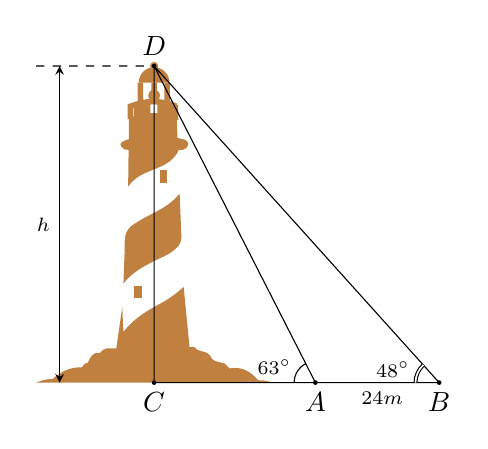
\begin{tikzpicture}[scale=.3,declare function={h=13.4;a=h/tan(63);b=h/tan(48);}]
			\fill[brown] (-5,0) 
			to[out=20,in=180] (-4.3,.15)
			to[out=40,in=180] (-3.05,.65)
			to[out=80,in=200] (-2.8,.85)
			to[out=70,in=160] (-2.3,1.25)
			to[out=50,in=190] (-2,1.45)
			--(-1.6,1.45)--(-1.35,3.2)--(-1.3,2.15)
			to[out=50,in=210] (0,3.2)
			to[out=28,in=222] (1.25,4.05)
			--(1.5,1.5)--(1.7,1.5)
			to[out=-40,in=180] (2,1.33)
			to[out=-10,in=110] (2.45,1)
			to[out=-40,in=160] (3,.8)
			to[out=-40,in=150] (3.2,.6)
			to[out=10,in=130] (4.4,.1)
			to[out=0,in=160] (5,0)
			--cycle;
			\fill[brown] (-.85,3.6) rectangle (-.53,4.1);
			\fill[brown] (-1.3,4.2)
			to[out=50,in=208] (0,5.15)
			to[out=25,in=225] (1,5.75)
			to[out=50,in=275] (1.15,6.3)
			--(1.08,8)
			to[out=-130,in=37] (-1,6.6)
			to[out=-135,in=88] (-1.25,5.5)
			--cycle;
			\fill[brown] (.25,8.45) rectangle (.55,9);
			\fill[brown] (-1.1,8.3)
			to[out=55,in=245] (1.05,9.85)--(1.2,9.85)
			to[out=10,in=263] (1.45,10.1)
			to[out=100,in=-10] (.99,10.35)--(.96,11.1)--(1.05,11.15)
			to[out=155,in=20] (-1.07,11.2)--(-1.07,10.3)
			to[out=-175,in=135] (-1.4,10)
			to[out=-55,in=190] (-1.08,9.85)--cycle;
			\draw[brown,line width= 2pt] 
			(.9,11.15)--(.9,11.75)
			(.25,11.35)--(.25,11.9)
			(-.28,11.35)--(-.28,11.9)
			(-1,11.15)--(-1,11.7)
			to[out=20,in=160] (0.94,11.7)
			(.55,11.8)--(.55,12.7)
			(-.58,11.8)--(-.58,12.7)
			(0,11.9)--(0,12.7);
			\draw[brown,line width=4pt] 
			(.6,11.25)--(.6,11.8)
			(-.63,11.25)--(-.63,11.8);
			\fill[brown] (0,12.15) circle (7pt)
			(.65,12.7) arc (0:180:.65) -- cycle
			(0,13.4) circle (5pt);
			\path 
			(0,0) coordinate (C)
			(a,0) coordinate (A)
			(b,0) coordinate (B)
			(0,h) coordinate (D);
			\foreach \i/\g in {C/-90, A/-90, B/-90, D/90} \fill (\i)circle(.1) node[shift={(\g:.25)}] {$\i$};
			\draw (C)--(B)node[pos=.8, below]{\scriptsize$24m$}--(D)--cycle (A)--(D)
			(A)+(-.9,0) arc (180:117:.9)node[pos=.75, left]{\scriptsize$63^\circ$};
			\draw[double] (B)+(-1,0) arc (180:132:1)node[pos=.7, left]{\scriptsize$48^\circ$};
			\draw[dashed] (-5,h)--(D);
			\draw[stealth-stealth] (-4,0) -- (-4,h)node[pos=.5, left]{\scriptsize$h$};
	\end{tikzpicture}}
\loigiai{
\begin{center}
	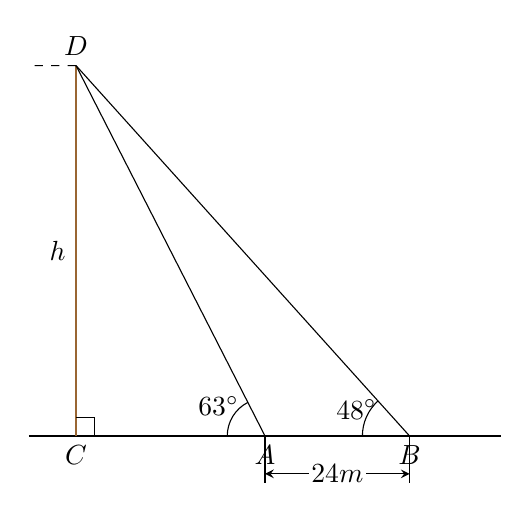
\begin{tikzpicture}[>=stealth, scale=1.2]
		% Định nghĩa các toạ độ theo đúng tỉ lệ lượng giác
		\coordinate (C) at (0,0);
		\coordinate (D) at (0, 3.92); % Giả sử AC = 2 -> CD = 2*tan(63) = 3.92
		\coordinate (A) at (2,0);
		\coordinate (B) at (3.53,0); % CB = CD/tan(48) = 3.92/tan(48) = 3.53
		
		% Vẽ mặt đất và tháp
		\draw[thick] (-0.5,0) -- (4.5,0);
		\draw[thick, brown!80!black] (C) -- (D) node[midway, left, text=black] {$h$};
		
		% Vẽ các tia nhìn
		\draw (A) -- (D);
		\draw (B) -- (D);
		
		% Vẽ đường gióng ngang trên đỉnh tháp
		\draw[dashed] (D) -- (-0.5, 3.92);
		
		% Gắn tên điểm
		\node[below] at (C) {$C$};
		\node[above] at (D) {$D$};
		\node[below] at (A) {$A$};
		\node[below] at (B) {$B$};
		
		% Đánh dấu đoạn AB
		\draw[<->] (A) ++(0,-0.4) -- (B |- {0,-0.4}) node[midway, fill=white, inner sep=1pt] {$24\text{ m}$};
		\draw (A) -- ++(0,-0.5);
		\draw (B) -- ++(0,-0.5);
		
		% Ký hiệu góc vuông
		\draw (0.2,0) |- (0,0.2);
		
		% Ký hiệu góc 63 độ
		\draw (A) ++(-0.4,0) arc (180:117:0.4);
		\node at ([xshift=-14pt, yshift=9pt]A) {$63^\circ$};
		
		% Ký hiệu góc 48 độ
		\draw (B) ++(-0.5,0) arc (180:132:0.5);
		\node at ([xshift=-16pt, yshift=8pt]B) {$48^\circ$};
	\end{tikzpicture}
\end{center}

Xét tam giác $ABD$, ta có $\widehat{CAD}$ là góc ngoài tại đỉnh $A$ của tam giác, do đó:
$$ \widehat{CAD} = \widehat{ABD} + \widehat{ADB} $$
Suy ra $\widehat{ADB} = \widehat{CAD} - \widehat{ABD} = 63^\circ - 48^\circ = 15^\circ$.

Áp dụng định lí sin trong tam giác $ABD$, ta có:
$$ \dfrac{AD}{\sin \widehat{ABD}} = \dfrac{AB}{\sin \widehat{ADB}} \Rightarrow \dfrac{AD}{\sin 48^\circ} = \dfrac{24}{\sin 15^\circ} $$
Suy ra:
$$ AD = \dfrac{24 \cdot \sin 48^\circ}{\sin 15^\circ} \text{ (m)}. $$

Xét tam giác $ACD$ vuông tại $C$, áp dụng tỉ số lượng giác, ta có:
$$ \sin \widehat{CAD} = \dfrac{CD}{AD} \Rightarrow h = CD = AD \cdot \sin 63^\circ $$

Thay giá trị của $AD$ vừa tìm được vào biểu thức trên, ta được:
$$ h = \dfrac{24 \cdot \sin 48^\circ \cdot \sin 63^\circ}{\sin 15^\circ} \approx 61{,}4 \text{ (m)}. $$

Vậy chiều cao $h$ của khối tháp xấp xỉ $61{,}4 \text{ m}$.}
\end{vd}
\dongcham{3}
\begin{vd}
	\immini{Để tránh núi, đường giao thông hiện tại phải đi vòng $A \rightarrow B \rightarrow C \rightarrow D$ như mô hình trong hình bên. Để rút ngắn khoảng cách và tránh sạt lở núi, người ta dự định làm đường hàm xuyên núi, nối thẳng từ $A$ tới $D$. Hỏi độ dài đường mới sẽ giảm bao nhiêu kilômét so với đường cũ?
}{
\begin{tikzpicture}[thick, font=\small, scale=1]
	\def\k{1.7}
	\def\pica{\begin{tikzpicture}
			\path (0,0)coordinate(A1) ++(50:\k)coordinate(A2)++(-45:1.1*\k)coordinate(A3) 
			($(A1)!0.8!(A2)$)coordinate(A12) 
			($(A3)!0.8!(A2)$)coordinate(A23)
			($(A12)!0.3!(A23)$)coordinate(A4)
			($(A12)!0.7!(A23)$)coordinate(A5)
			;
			\shadedraw [left color = cyan!60!white, right color = cyan!30!white!50!black, draw=black] (A1) to [controls=+(20:0.1*\k) and +(-130:0.1*\k)] (A12) to [controls=+(50:0.2*\k) and +(130:0.2*\k)] (A23) to [controls=+(-45:0.1*\k) and +(160:0.2*\k)] (A3) %%
			(A1) to [controls=+(-110:0.05*\k) and +(-130:0.1*\k)] ($($(A1)!0.2!(A3)$)+(-90:0.15*\k)$)coordinate(B1)
			to [controls=+(-80:0.1*\k) and +(-100:0.1*\k)] ($($(A1)!0.7!(A3)$)+(-90:0.18*\k)$)coordinate(B2)
			to [controls=+(-80:0.05*\k) and +(-80:0.1*\k)] (A3)
			;
			\fill [white, draw=black]  (A12) to [controls=+(50:0.2*\k) and +(130:0.2*\k)] (A23) to [controls=+(195:0.15*\k) and +(-30:0.1*\k)] (A12);
			\draw ($(B1)!0.1!(A4)$) to [controls=+(50:0.1*\k) and +(-120:0.1*\k)] ($(B1)!0.6!(A4)$) ($(B2)!0.2!(A5)$)  to [controls=+(130:0.1*\k) and +(-80:0.1*\k)] ($(B2)!0.8!(A5)$);
		\end{tikzpicture}
	}
	\draw (3.5,-0.4)node{\pica};
	\def\k{2}\draw (0,0)node{\pica};
	\def\k{3}
	\draw (2,-1)node{\pica};
	\draw [line width=8pt, black,rounded corners ] (-2.5,-0.5)coordinate(C1) -- (-2,-0.5)coordinate(C2) -- (0.8,-3)coordinate(C3) -- (3.7,-3)coordinate(C4) -- (5.2,-0.5)coordinate(C5) -- (6,-0.5)coordinate(C6) ;
	\draw [dashed, line width=1pt, yellow,rounded corners , shift=(-90:0pt)] (C1)--(C2)--(C3)--(C4)--(C5)--(C6);
	\path (C5)node[above=5pt]{\Large $\mathbf{A}$}
	(C4)node[below right=5pt]{\Large $\mathbf{B}$}node[shift={(130:17pt)}]{\Large $\mathbf{100^\circ}$}
	(C3)node[below left=5pt]{\Large $\mathbf{C}$}node[shift={(50:17pt)}]{\Large $\mathbf{145^\circ}$}
	(C2)node[above=5pt]{\Large $\mathbf{D}$}
	(C5)--(C4)node[midway, right=5pt]{\Large $\mathbf{6\ km}$}
	(C4)--(C3)node[midway, below=5pt]{\Large $\mathbf{5\ km}$}
	(C2)--(C3)node[midway, left=5pt]{\Large $\mathbf{10\ km}$};
\end{tikzpicture}}
	\loigiai{\begin{center}
			\begin{tikzpicture}[>=stealth, scale=0.6]
				% Định nghĩa các toạ độ để mô phỏng hình vẽ
				\coordinate (C) at (0,0);
				\coordinate (B) at (5,0);
				% Góc CBA = 100 độ, nên BA tạo với tia đối của BC một góc 80 độ
				\coordinate (A) at (6.04, 5.91); 
				% Góc BCD = 145 độ
				\coordinate (D) at (-8.19, 5.74); 
				
				% Vẽ các đoạn đường cũ
				\draw[line width=4pt, black] (D) -- (C) -- (B) -- (A);
				\draw[line width=1pt, dashed, yellow] (D) -- (C) node[midway, below left, text=black] {\bf $10$ km};
				\draw[line width=1pt, dashed, yellow] (C) -- (B) node[midway, below, text=black] {\bf $5$ km};
				\draw[line width=1pt, dashed, yellow] (B) -- (A) node[midway, right, text=black] {\bf $6$ km};
				
				% Vẽ đường hầm mới và đường chéo phụ
				\draw[dashed, thick, red] (D) -- (A) node[midway, above] {Đường hầm};
				\draw[thin, blue] (A) -- (C);
				
				% Tên các điểm
				\node[above right, font=\bfseries] at (A) {A};
				\node[below right, font=\bfseries, yshift=-5pt] at (B) {B};
				\node[below left, font=\bfseries, yshift=-5pt] at (C) {C};
				\node[above left, font=\bfseries] at (D) {D};
				
				% Ký hiệu góc
				\draw (B) ++(-0.6,0) arc (180:80:0.6);
				\node[font=\bfseries] at (4.1, 0.5) {$100^\circ$};
				
				\draw (0.6,0) arc (0:145:0.6);
				\node[font=\bfseries] at (0.3, 0.7) {$145^\circ$};
			\end{tikzpicture}
		\end{center}
		
		Nối $A$ và $C$, xét $\triangle ABC$, áp dụng định lí côsin, ta có:
		\begin{align*}
			AC^2 &= AB^2 + BC^2 - 2 \cdot AB \cdot BC \cdot \cos \widehat{ABC} \\
			&= 6^2 + 5^2 - 2 \cdot 6 \cdot 5 \cdot \cos 100^\circ \\
			&= 61 - 60 \cos 100^\circ \approx 71{,}42
		\end{align*}
		Suy ra $AC \approx 8{,}45 \text{ (km)}$.
		
		Tiếp tục áp dụng hệ quả định lí côsin trong $\triangle ABC$ để tìm góc $\widehat{BCA}$:
		$$ \cos \widehat{BCA} = \dfrac{BC^2 + AC^2 - AB^2}{2 \cdot BC \cdot AC} \approx \dfrac{5^2 + 71{,}42 - 6^2}{2 \cdot 5 \cdot 8{,}45} = \dfrac{60{,}42}{84{,}5} \approx 0{,}715 $$
		Suy ra $\widehat{BCA} \approx 44{,}36^\circ$.
		
		Ta có: $\widehat{ACD} = \widehat{BCD} - \widehat{BCA} \approx 145^\circ - 44{,}36^\circ = 100{,}64^\circ$.
		
		Xét $\triangle ACD$, áp dụng định lí côsin, ta có:
		\begin{align*}
			AD^2 &= AC^2 + CD^2 - 2 \cdot AC \cdot CD \cdot \cos \widehat{ACD} \\
			&\approx 71{,}42 + 10^2 - 2 \cdot 8{,}45 \cdot 10 \cdot \cos 100{,}64^\circ \\
			&\approx 171{,}42 - 169 \cdot (-0{,}1846) \\
			&\approx 171{,}42 + 31{,}20 = 202{,}62
		\end{align*}
		Suy ra $AD \approx \sqrt{202{,}62} \approx 14{,}23 \text{ (km)}$.
		
		Độ dài đường giao thông cũ đi vòng là:
		$$ S_{c\tilde{u}} = AB + BC + CD = 6 + 5 + 10 = 21 \text{ (km)}. $$
		
		Khoảng cách đường mới giảm đi so với đường cũ là:
		$$ \Delta S = S_{c\tilde{u}} - AD \approx 21 - 14{,}23 = 6{,}77 \text{ (km)}. $$
		
		Vậy độ dài đường mới làm hầm xuyên núi sẽ giảm khoảng $6{,}77 \text{ km}$ so với đường cũ.}
\end{vd}
\dongcham{5}
\begin{vd}
	\immini{Một tàu đánh cá xuất phát từ cảng $A$ , đi theo hướng $\rm{S6}0^\circ{\rm{E}}$ với vận tốc $80\rm{km/h}$ . Đi được 2 giờ thì động cơ của tàu bị hỏng nên tàu trôi tự do theo hướng nam với vận tốc $\rm{7 km/h}$ . Sau 90 phút kể từ khi động cơ bị hỏng, tàu neo đậu được vào một hòn đảo.
		\begin{tasks}(1)
			\task Tính khoảng cách từ cảng $A$ tới đảo nơi tàu neo đậu.
			\task Xác định hướng từ cảng $A$ tới đảo nơi tàu neo đậu.
		\end{tasks}
		\dapso{a) $165,5$ km. \quad \quad b) $\rm{S56}^\circ 50'{\rm{E}}$.}}{
		\begin{tikzpicture}[smooth,font=\footnotesize,scale=0.5,>=latex]
			\path
			(0,0) coordinate (O)
			(4,0) coordinate (E)
			(-4,0) coordinate (W)
			(0,-5.5) coordinate (S)
			(0,2) coordinate (N)
			(3,-1) coordinate (S1)
			(3,-4) coordinate (B)
			;
			\draw[fill=black]
			(O) circle (2.5pt) (S1) circle (2.5pt) (B) circle (2.5pt)
			(3,-1)--(3,-4) node[below]{\scriptsize$B$};
			\draw[dashed] (B)--(O);
			\draw[line width=1pt,black,<->] (W)node[left]{\scriptsize$W$ (Tây)}--(E)node[right]{\scriptsize$E$ (Đông)};
			\draw[line width=0.7pt,black,<->] (S)node[below]{\scriptsize$S$ (Nam)}--(N)node[above]{\scriptsize$N$ (Bắc)};
			\draw[line width=0.7pt,->] (O)node[above left]{\scriptsize$A$}--(S1)node[right]{\scriptsize$S\alpha^\circ E$};
			\draw
			pic["\scriptsize$60^\circ$",angle radius=11mm]{angle = S--O--S1}
			pic[draw,angle radius=3mm]{angle = S--O--S1}
			;
	\end{tikzpicture}}
	\loigiai{
		Sau 2 giờ, tàu cá chạy từ $A$ đến $B$ với vận tốc $80\rm{km/h}$ , nên $AB=2.80=160$ (km).\\
		Sau 90 phút, tàu trôi từ $B$ đến $C$ với vận tốc $\rm{7 km/h}$ , suy ra $BC=7.1,5=10,5$ (km).\\
		Vì từ $A$ đến $B$ tàu chạy theo hướng $\rm{S6}0^\circ{\rm{E}}$ và từ $B$ đến $C$ tàu trôi theo hướng $\rm{S}0^\circ{\rm{E}}$ , nên $\widehat{ABC}=180^\circ-60^\circ=120^\circ $ .
		\begin{enumerate}[a)]
			\item Theo định lí côsin, ta có\\
			$A{C^2}=A{B^2}+B{C^2}-2AB.BC.\cos\widehat{ABC}=27390,25\Rightarrow AC=165,5$ (km).\\
			Vậy khoảng cách từ cảng $A$ tới đảo nơi tàu neo đậu là $165,5$ km.
			\item Gọi hướng từ cảng $A$ tới đảo nơi tàu neo đậu $C$ là hướng $\rm{S}x^\circ{\rm{E}}$ . Khi đó, do $BC{\rm{//}}AS$ nên $\widehat{SAC}=\widehat{ACB}=x$ .\\
			Áp dụng định lí sin trong tam giác $ABC$ , ta có:\\
			$\dfrac{AC}{\sin B}=\dfrac{AB}{\sin C}\Rightarrow\sin C=\dfrac{AB.\sin B}{AC}=\dfrac{160.\sin 120^\circ}{165,5}\approx 0,8372\Rightarrow x=\widehat C\approx 56^\circ 50'$ .\\
			Vậy hướng từ cảng $A$ tới đảo nơi tàu neo đậu là $\rm{S56}^\circ 50'{\rm{E}}$
		\end{enumerate}
}
\end{vd}
\dongcham{10}
\boxmini{BÀI TẬP TỔNG HỢP TỰ LUYỆN}

\begin{baitap}
	Giải tam giác $ABC$, biết:
	\begin{enumEX}[a)]{2}
		\item $a = b = 6; \widehat{C} = 54^\circ$.
		\item $c = 7; b = 23; \widehat{A} = 130^\circ$.
		\item $c = 14; \widehat{A} = 60^\circ; \widehat{B} = 40^\circ$.
		\item $b = 35; \widehat{A} = 40^\circ; \widehat{C} = 120^\circ$.
		\item $a = 14; b = 18; c = 20$.
		\item $a = 6; b = 7{,}3; c = 4{,}8$.
	\end{enumEX}
	\loigiai{
		\begin{enumerate}
			\item[a)] Ta có $a = b = 6$ nên tam giác $ABC$ cân tại $C$.
			Suy ra $\widehat{A} = \widehat{B} = \dfrac{180^\circ - \widehat{C}}{2} = \dfrac{180^\circ - 54^\circ}{2} = 63^\circ$.
			
			Áp dụng định lí côsin trong tam giác $ABC$, ta có:
			\begin{align*}
				c^2 &= a^2 + b^2 - 2ab \cos C \\
				&= 6^2 + 6^2 - 2 \cdot 6 \cdot 6 \cdot \cos 54^\circ \\
				&= 72 - 72 \cos 54^\circ \approx 29{,}68.
			\end{align*}
			Suy ra $c \approx \sqrt{29{,}68} \approx 5{,}45$.
			
			\item[b)] Áp dụng định lí côsin trong tam giác $ABC$, ta có:
			\begin{align*}
				a^2 &= b^2 + c^2 - 2bc \cos A \\
				&= 23^2 + 7^2 - 2 \cdot 23 \cdot 7 \cdot \cos 130^\circ \\
				&\approx 529 + 49 - 322 \cdot (-0{,}6428) \approx 784{,}98.
			\end{align*}
			Suy ra $a \approx \sqrt{784{,}98} \approx 28{,}02$.
			
			Áp dụng định lí sin, ta có:
			$$ \dfrac{a}{\sin A} = \dfrac{b}{\sin B} \Rightarrow \sin B = \dfrac{b \sin A}{a} \approx \dfrac{23 \cdot \sin 130^\circ}{28{,}02} \approx 0{,}6288 \Rightarrow \widehat{B} \approx 38^\circ 58'. $$
			Suy ra $\widehat{C} = 180^\circ - (\widehat{A} + \widehat{B}) \approx 180^\circ - (130^\circ + 38^\circ 58') = 11^\circ 2'$.
			
			\item[c)] Xét tam giác $ABC$, ta có:
			$$ \widehat{C} = 180^\circ - (\widehat{A} + \widehat{B}) = 180^\circ - (60^\circ + 40^\circ) = 80^\circ. $$
			
			Áp dụng định lí sin $\dfrac{a}{\sin A} = \dfrac{b}{\sin B} = \dfrac{c}{\sin C}$, ta có:
			\begin{itemize}
				\item $a = \dfrac{c \sin A}{\sin C} = \dfrac{14 \cdot \sin 60^\circ}{\sin 80^\circ} \approx 12{,}31$.
				\item $b = \dfrac{c \sin B}{\sin C} = \dfrac{14 \cdot \sin 40^\circ}{\sin 80^\circ} \approx 9{,}14$.
			\end{itemize}
			
			\item[d)] Xét tam giác $ABC$, ta có:
			$$ \widehat{B} = 180^\circ - (\widehat{A} + \widehat{C}) = 180^\circ - (40^\circ + 120^\circ) = 20^\circ. $$
			
			Áp dụng định lí sin $\dfrac{a}{\sin A} = \dfrac{b}{\sin B} = \dfrac{c}{\sin C}$, ta có:
			\begin{itemize}
				\item $a = \dfrac{b \sin A}{\sin B} = \dfrac{35 \cdot \sin 40^\circ}{\sin 20^\circ} \approx 65{,}78$.
				\item $c = \dfrac{b \sin C}{\sin B} = \dfrac{35 \cdot \sin 120^\circ}{\sin 20^\circ} \approx 88{,}63$.
			\end{itemize}
			
			\item[e)] Áp dụng hệ quả của định lí côsin, ta có:
			\begin{itemize}
				\item $\cos A = \dfrac{b^2 + c^2 - a^2}{2bc} = \dfrac{18^2 + 20^2 - 14^2}{2 \cdot 18 \cdot 20} = \dfrac{528}{720} = \dfrac{11}{15} \Rightarrow \widehat{A} \approx 42^\circ 50'$.
				\item $\cos B = \dfrac{a^2 + c^2 - b^2}{2ac} = \dfrac{14^2 + 20^2 - 18^2}{2 \cdot 14 \cdot 20} = \dfrac{272}{560} = \dfrac{17}{35} \Rightarrow \widehat{B} \approx 60^\circ 56'$.
			\end{itemize}
			Suy ra $\widehat{C} = 180^\circ - (\widehat{A} + \widehat{B}) \approx 180^\circ - (42^\circ 50' + 60^\circ 56') = 76^\circ 14'$.
			
			\item[f)] Tương tự, áp dụng hệ quả của định lí côsin, ta có:
			\begin{itemize}
				\item $\cos A = \dfrac{b^2 + c^2 - a^2}{2bc} = \dfrac{7{,}3^2 + 4{,}8^2 - 6^2}{2 \cdot 7{,}3 \cdot 4{,}8} = \dfrac{40{,}33}{70{,}08} \approx 0{,}5755 \Rightarrow \widehat{A} \approx 54^\circ 52'$.
				\item $\cos B = \dfrac{a^2 + c^2 - b^2}{2ac} = \dfrac{6^2 + 4{,}8^2 - 7{,}3^2}{2 \cdot 6 \cdot 4{,}8} = \dfrac{5{,}75}{57{,}6} \approx 0{,}0998 \Rightarrow \widehat{B} \approx 84^\circ 16'$.
			\end{itemize}
			Suy ra $\widehat{C} = 180^\circ - (\widehat{A} + \widehat{B}) \approx 180^\circ - (54^\circ 52' + 84^\circ 16') = 40^\circ 52'$.
		\end{enumerate}
	}
\end{baitap}

\begin{baitap}
	Cho $\Delta ABC$ có $\widehat{A}=90^\circ$, bán kính đường tròn ngoại tiếp $R=7$ và bán kính đường tròn nội tiếp là $r=3$. Tính diện tích $S$ của tam giác.
	\loigiai{
		Gọi $I$ là tâm đường tròn nội tiếp của $\Delta ABC$.
		\\ Gọi tiếp điểm của đường tròn nội tiếp $(I)$ với các cạnh $BC,CA, AB$ lần lượt là $D,E,F$.
		\\ Vì $\Delta ABC$ vuông tại A nên $BC=2R=14$ và $AE=AF=r=3$.
		\\ Ta có $p=\dfrac{AB+AC+BC}{2}=AE+BC=14+3=17$
		\\ Vậy $S=pr=17\cdot 3=51$}
\end{baitap}\cham{12}

\begin{baitap}%[0H2B3-4]
	\immini
	{
		Để đo khoảng cách từ vị trí $A$ đến vị trí $B$ ở hai bên bờ một cái ao, bạn An đi dọc bờ ao từ vị trí $A$ đến vị trí $C$ và tiến hành đo các góc $BAC$, $BCA$. Biết $AC=25 \text{ m}$, $\widehat{BAC}=59{,}95^\circ$, $\widehat{BCA}=82{,}15^\circ$ (hình vẽ bên). Hỏi khoảng cách từ vị trí $A$ đến vị trí $B$ là bao nhiêu mét (làm tròn kết quả đến hàng đơn vị)?
		\cham{8}
	}
	{
		\begin{tikzpicture}[scale=1,font=\footnotesize,line cap=round,line join=round,>=stealth]
			\def\a{3.75}
			\path (0:0) coordinate(A) (59.95:1) coordinate(a) (0:\a) coordinate(C)  + (97.85:1) coordinate(c)  (intersection of A--a and C--c) coordinate(B);
			\fill[cyan!60] (-.5,2) .. controls +(-70:2) and +(150:1) .. (2.5,1) .. controls +(-15:2) and +(-30:1) .. (4.5,3.5) .. controls +(150:1) and +(40:1) .. (2,4) .. controls +(-150:1.5) and +(100:2) .. cycle;
			\draw (A)--(B)--(C)--cycle;
			\foreach \d/\g in {A/-135, B/90, C/-45}
			\fill (\d) circle(1pt) node[shift={(\g:.3)}]{$\d$};
			\path (A)--(C) node[midway,below]{$25$ m} pic[draw,angle radius=.3cm]{angle=C--A--B} (A) node[shift={(20:.8)}]{$59{,}95^\circ$} pic[draw,angle radius=.3cm]{angle=B--C--A} pic[draw,angle radius=.35cm]{angle=B--C--A} (C) node[shift={(150:.7)}]{$82{,}15^\circ$};
			
		\end{tikzpicture}
	}
	\loigiai
	{
		Trong tam giác $ABC$ ta có
		\[\widehat{A}+\widehat{B}+\widehat{C}=180^\circ \Rightarrow \widehat{B}=180^\circ - \left(\widehat{A}+\widehat{C}\right) \Rightarrow \widehat{B} = 180^\circ - \left(59{,}95^\circ + 82{,}15^\circ\right) = 37{,}9^\circ.\]
		Áp dụng định lí sin trong tam giác $ABC$ ta có
		\[\dfrac{AB}{\sin C} = \dfrac{AC}{\sin B} \Rightarrow AB = \dfrac{AC\sin C}{\sin B} = \dfrac{25\sin 82{,}15^\circ}{\sin 59{,}95^\circ} \approx 29 \text{ m}.\]
		Vậy khoảng cách từ vị trí $A$ đến vị trí $B$ gần bằng $29$ mét.
	}
\end{baitap}

\begin{baitap}
	\immini{Trên nóc một tòa nhà có một cột ăng-ten cao $7 \mathrm{~m}$. Từ một vị trí quan sát $A$ cao $10 \mathrm{~m}$ so với mặt đất có thể nhìn thấy định $B$ và chân $C$ của cột ăng-ten, với các góc tương ứng là $75^{\circ}$ và $45^{\circ}$ so với phương nằm ngang.
		\begin{tasks}(1)
			\task Tính các góc của tam giác $A B C$.
			\task Tính chiều cao của tòa nhà.
		\end{tasks}
	}{
		\begin{tikzpicture}[scale=1, font=\footnotesize,>=stealth]
			\path 
			(0,0) coordinate (A)
			(4,3) coordinate (C)
			(4,4) coordinate (B)
			(4,-1) coordinate (O) 
			(0,-1) coordinate (L) 
			(4,0) coordinate (R) 
			;
			\draw[dashed] (A)--(B) (A)--(C);
			\draw[thick](B)--(C);
			\draw[fill=cyan] (C)--(6,3)--(6,-1)--(4,-1)--(C);
			\foreach \i in {2,3,4,5}
			\draw[fill=white] ({4+1/3},{-1+(2/3)*(\i-1)})--({4+1/3},{-1+(2/3)*(\i-1)+0.5})--({4+2/3},{-1+(2/3)*(\i-1)+0.5})--({4+2/3},{-1+(2/3)*(\i-1)})--cycle 
			({5+1/3},{-1+(2/3)*(\i-1)})--({5+1/3},{-1+(2/3)*(\i-1)+0.5})--({5+2/3},{-1+(2/3)*(\i-1)+0.5})--({5+2/3},{-1+(2/3)*(\i-1)})--cycle;
			\draw[dashed]   (A)--(R); 
			\draw [<->](A)--(L);
			\draw ($(A)!0.5!(L)$) node[left]{$10 \mathrm{~m}$} ($(B)!0.5!(C)$) node[right]{\scriptsize$7 \mathrm{~m}$} ;
			\draw pic["\scriptsize$75^{\circ}$", draw=black, angle eccentricity=1.4, angle radius=1.1cm]{angle=R--A--B};
			\draw pic["\scriptsize$45^{\circ}$", draw=black,double, angle eccentricity=1.4, angle radius=0.6cm]{angle=R--A--C};
			\foreach \x/\g in {A/180,B/140,C/140} 
			\fill[black] (\x) circle (1pt)+(\g:3mm) node {$\x$};
			\clip (-0.5,{-1-0.25}) rectangle (6.6,-1) ;
			\draw[fill=gray!30] (-0.5,-1)--(6.6,-1)--(6.6,{-1-0.25})--(-0.5,{-1-0.25})--cycle;
			\foreach \i in {1,2,...,35}
			\draw ({-0.5+0.2*(\i)},-1)--($({-0.5+0.2*(\i)},-1)+(-120:0.3)$) ;
	\end{tikzpicture}}
\loigiai{
Gọi $H$ là hình chiếu vuông góc của $A$ lên đường thẳng chứa cột ăng-ten $BC$. Đường thẳng $AH$ là phương nằm ngang.
Theo giả thiết, ta có $\widehat{HAC} = 45^\circ$ và $\widehat{HAB} = 75^\circ$.

\begin{enumerate}
	\item[a)] \textbf{Tính các góc của tam giác $ABC$:}
	\begin{itemize}
		\item Ta có $\widehat{BAC} = \widehat{HAB} - \widehat{HAC} = 75^\circ - 45^\circ = 30^\circ$.
		\item Xét tam giác $AHB$ vuông tại $H$, ta có:
		$$ \widehat{ABH} = 90^\circ - \widehat{HAB} = 90^\circ - 75^\circ = 15^\circ $$
		Do ba điểm $B, C, H$ thẳng hàng nên $\widehat{ABC} = \widehat{ABH} = 15^\circ$.
		\item Xét tam giác $ABC$, tổng ba góc bằng $180^\circ$, suy ra:
		$$ \widehat{ACB} = 180^\circ - (\widehat{BAC} + \widehat{ABC}) = 180^\circ - (30^\circ + 15^\circ) = 135^\circ $$
	\end{itemize}
	Vậy tam giác $ABC$ có các góc là $\widehat{A} = 30^\circ$, $\widehat{B} = 15^\circ$ và $\widehat{C} = 135^\circ$.
	
	\item[b)] \textbf{Tính chiều cao của tòa nhà:}
	Xét tam giác $AHC$ vuông tại $H$, ta có:
	$$ \tan \widehat{HAC} = \dfrac{CH}{AH} \Rightarrow \tan 45^\circ = \dfrac{CH}{AH} \Rightarrow CH = AH \quad (1) $$
	
	Xét tam giác $AHB$ vuông tại $H$, ta có:
	$$ \tan \widehat{HAB} = \dfrac{BH}{AH} \Rightarrow \tan 75^\circ = \dfrac{CH + BC}{AH} = \dfrac{CH + 7}{AH} \quad (2) $$
	
	Thế $(1)$ vào $(2)$, ta được:
	\begin{align*}
		& \tan 75^\circ = \dfrac{AH + 7}{AH} \\
		\Leftrightarrow\ & AH \cdot \tan 75^\circ = AH + 7 \\
		\Leftrightarrow\ & AH(\tan 75^\circ - 1) = 7 \\
		\Leftrightarrow\ & AH = \dfrac{7}{\tan 75^\circ - 1} 
	\end{align*}
	
	Sử dụng giá trị $\tan 75^\circ = 2 + \sqrt{3}$, ta tính được:
	$$ AH = \dfrac{7}{2 + \sqrt{3} - 1} = \dfrac{7}{\sqrt{3} + 1} = \dfrac{7(\sqrt{3} - 1)}{2} \approx 2{,}56 \text{ (m)}. $$
	
	Từ $(1)$ suy ra $CH = AH \approx 2{,}56 \text{ (m)}$.
	
	Chiều cao của tòa nhà (tính từ mặt đất đến điểm $C$) là:
	$$ h = CH + 10 \approx 2{,}56 + 10 = 12{,}56 \text{ (m)}. $$
	
	Vậy chiều cao của tòa nhà khoảng $12{,}56 \text{ m}$.
\end{enumerate}}
\end{baitap}

\begin{baitap}%[Phạm Tuấn]%[0H2B3-4]
	\immini{
		Để đo chiều cao $CH$ của một  tháp truyền hình, người ta chọn hai điểm quan sát $A$, $B$ trên mặt đất (hình vẽ).  Biết $\widehat{CAH} =51^\circ$, $\widehat{CBH} =66^\circ$ và $AB=75 \mathrm{~m}$, tính chiều cao của tháp.
		\cham{6}
	}
	{
		\begin{tikzpicture}[scale=1, font=\footnotesize, line join=round, line cap=round,>=stealth]
			\path
			(1,0) coordinate (A)
			(2,0) coordinate (B)
			(4,3.5) coordinate (C)
			(4,0) coordinate (H)
			(3.75,0) coordinate (U)
			(4.25,0) coordinate (V)
			;
			\draw[thick] (U)--(C)--(V); 
			\draw (B)--(C)--(A)--(V) ;
			\draw[dashed] (C)--(H) ;  
			\draw  
			($(C)!{1}!(U)$)--($(C)!{0.9}!(V)$)
			--($(C)!{0.8}!(U)$)--($(C)!{0.7}!(V)$)
			--($(C)!{0.6}!(U)$)--($(C)!{0.5}!(V)$)
			--($(C)!{0.4}!(U)$)--($(C)!{0.3}!(V)$)
			--($(C)!{0.2}!(U)$)--($(C)!{0.1}!(V)$)
			;
			
			\tkzMarkAngle[arc=l, size=0.6,mark=0](H,A,C)
			\tkzLabelAngle[pos=1](H,A,C) {$51^{\circ}$}
			\tkzMarkAngle[arc=ll, size=0.6,mark=0](H,B,C)
			\tkzLabelAngle[pos=1](H,B,C) {$66^{\circ}$}
			\foreach \x/\g in {A/-90,B/-90,C/90,H/-90} 
			\fill[black] (\x) circle (1pt)+(\g:3mm) node {$\x$};
		\end{tikzpicture}
	}
	
	\loigiai{
		Ta có $\widehat{ACB}=\widehat{CBH} - \widehat{CAH}=  66^\circ -51^\circ= 15^\circ$. \\
		Áp dụng định lí sin ta có
		\[
		\dfrac{AB}{\sin \widehat{ACB}} = \dfrac{BC}{\sin \widehat{CAH} } \Rightarrow BC = \dfrac{AB\sin \widehat{CAH}}{\sin \widehat{ACB}}  = \dfrac{75\sin 51^\circ}{\sin 15^\circ}.
		\]
		Suy ra $CH =BC\sin \widehat{CBH} = \dfrac{75 \sin 51^\circ \sin 66^\circ}{\sin 15^\circ} \approx 205{,}7\mathrm{~m}.$
	}
\end{baitap}\cham{7}

\begin{baitap}%[Phạm Tuấn]%[0H2B3-4]
	\immini{
		Trên ngọn đồi có một cái tháp cao $120 \mathrm{~m}$. Đỉnh tháp $B$ và chân tháp $C$ nhìn điểm $A$ ở chân đồi dưới các góc tương ứng bằng $35^{\circ}$ và $60^{\circ}$ so với phương thẳng đứng. Xác định chiều cao $H A$ của ngọn đồi. (Làm tròn đến phần mười).
		\cham{8}
	}
	{
		\begin{tikzpicture}[scale=1, font=\footnotesize, line join=round, line cap=round, >=stealth]
			\path 
			(0,0) coordinate (X)
			(1.1,2) coordinate (Y)
			(2,2) coordinate (Z)
			(5,0) coordinate (A)
			(1.5,5) coordinate (B)
			(1.5,2) coordinate (C)
			(1.5,0) coordinate (K)
			(1.3,2) coordinate (U)
			(1.8,2) coordinate (V) 
			(5,2) coordinate (H);
			\draw  
			($(B)!{1}!(U)$)--($(B)!{0.9}!(V)$)
			--($(B)!{0.8}!(U)$)--($(B)!{0.7}!(V)$)
			--($(B)!{0.6}!(U)$)--($(B)!{0.5}!(V)$)
			--($(B)!{0.4}!(U)$)--($(B)!{0.3}!(V)$)
			--($(B)!{0.2}!(U)$)--($(B)!{0.1}!(V)$)
			;
			\draw[thick]  (X)--(A)--(Z)--(Y)--(X);
			\draw (A)--(B)  (U)--(B)--(V) (Y)--($(Y)!{1.2}!(H)$)  (X)--($(X)!{1.2}!(A)$);
			\draw[->] (A)--(H) ; 
			\draw ($(A)!0.5!(H)$) node[right]{$h$};
			\draw[dashed](B)--(K) (A)--(C);
			
			\tkzMarkAngle[arc=l, size=0.6,mark=0](K,C,A)
			\tkzLabelAngle[pos=0.9](K,C,A) {$60^{\circ}$}
			\tkzMarkAngle[arc=ll, size=0.7,mark=0](K,B,A)
			\tkzLabelAngle[pos=1.1](V,B,A) {$35^{\circ}$}
			\foreach \x/\g in{A/-90,B/90,C/-130,H/90}
			\fill[black](\x) ($(\x)+(\g:3mm)$)node{$\x$}; 
		\end{tikzpicture}
	}
	\loigiai{
		Ta có $\widehat{BAC} = 60^\circ - 35^\circ =25^\circ $;  $\widehat{ACH} = 90^\circ - 60^\circ =30^\circ $\\
		Áp dụng định lí sin ta có
		\[
		\dfrac{AC}{\sin \widehat{ABC}} = \dfrac{BC}{\sin \widehat{BAC}} \Rightarrow AC =  \dfrac{BC\sin \widehat{ABC}}{\sin \widehat{BAC}}
		= \dfrac{120\sin 35^\circ}{\sin 25^\circ}.
		\]
		Suy ra $AH =AC \sin \widehat{ACH} = \dfrac{120 \sin 35^\circ \sin 30^\circ }{\sin 25^\circ} \approx 81{,}4 \mathrm{~m}$.
	}
\end{baitap}
\cham{4}

\begin{baitap}%[0H2K3-4]
	\immini
	{
		Bạn $A$ đứng ở đỉnh của tòa nhà và quan sát chiếc diều, nhận thấy góc nâng (góc nghiêng giữa phương từ mắt của bạn $A$ tới chiếc diều và phương nằm ngang) là $\alpha=35^\circ$; khoảng cách từ đỉnh tòa nhà tới mắt bạn $A$ là $1{,}5 \text{ m}$. Cùng lúc đó ở dưới chân tòa nhà, bạn $B$ cũng quan sát chiếc diều và thấy góc nâng là $\beta=75^\circ$; khoảng cách từ mặt đất tới mắt bạn $B$ cũng là $1{,}5 \text{ m}$. Biết chiều cao của tòa nhà là $h=20\text{ m}$ (minh họa ở hình bên). Chiếc diều bay cao bao nhiêu mét so với mặt đất (làm tròn kết quả đến hàng đơn vị)?
			}
	{
		\begin{tikzpicture}[scale=.8,font=\footnotesize,line cap=round,line join=round,>=stealth]
			\draw (0,0) coordinate(O)grid (2,6);
			\draw (2,6)--(2,6.5) coordinate(A) (2,.5) coordinate(B);
			\path[shift={(B)}] (75:1) coordinate(b);
			\path[shift={(A)}] (35:1) coordinate(a);
			\path (intersection of A--a and B--b) coordinate(C) ($(A)!.8!(C)$) coordinate(D) ($(O)!(C)!(5,0)$) coordinate(H) ($(C)!(A)!(H)$) coordinate(I) ($(C)!(B)!(H)$) coordinate(J);
			\path[shift={(C)}] (65:.4) coordinate(E) (140:1) coordinate(F) ($(C)!.6!(F)$) coordinate(G);
			\fill[cyan!80] (C)--(D) .. controls + (130:.5) and +(-100:.3) .. (F) .. controls +(10:.3) and +(120:.4) ..(E) .. controls +(-120:.3) and +(70:.2) .. cycle;
			\fill[blue!80!black] (C)--(G) .. controls +(50:.3) and +(130:.2) .. (E) .. controls +(-120:.3) and +(70:.2) .. cycle;
			\fill[blue!80!black] (D) .. controls + (130:.5) and +(-100:.3) .. (F) -- (G) .. controls +(-130:.3) and +(110:.2) .. cycle;
			\draw[color=blue!80!red] (C) .. controls +(-10:.6) and +(150:.5) .. (5,7);
			\draw[color=blue!80!red] (C) .. controls +(-15:.6) and +(150:.5) .. (4.8,6.9);
			\draw (A)--(C)--(B) (2,0)--(H);
			\draw[dashed] (C)--(H) (A)--(I) (B)--(J);
			\path (O)--(0,6) node[midway,left]{$h$} (A) node[shift={(180:.3)}]{$A$} (B) node[shift={(-45:.3)}]{$B$};
			\begin{scope}
				\clip (C)--(A)--(I);
				\draw (A) circle(.4) node[shift={(15:.5)}]{$\alpha$};
			\end{scope}
			\begin{scope}
				\clip (C)--(B)--(J);
				\draw[double] (B) circle(.4) node[shift={(35:.55)}]{$\beta$};
			\end{scope}
			
		\end{tikzpicture}
	}
	\loigiai
	{
		\immini
		{
			Kí hiệu $C$ là vị trí của chiếc diều.\\
			Từ điểm $B$ vẽ đường thẳng $Bx$ vuông góc với $AB$.\\
			Từ điểm $C$ kẻ $CH\perp Bx$ ($H$ thuộc $Bx$).\\
			Từ điểm $A$ kẻ $AK\perp CH$ ($K$ thuộc $CH$).\\
			Khi đó $\widehat{CAK}=\alpha$ và $\widehat{CBH}=\beta$.\\
			Chiều cao của diều so với mặt đất chính là độ dài đoạn thẳng $CH$.\\
			Vì khoảng cách từ đỉnh tòa nhà tới mắt bạn $A$ và khoảng cách từ mặt đất tới mắt bạn $B$ đều là $1{,}5 \text{ m}$ nên $AB=h=20\text{ m}$.\\
			Tứ giác $ABHK$ là hình chữ nhật.\\
			$\widehat{CAB} = \widehat{CAK}+\widehat{KAB} = 35^\circ + 90^\circ = 125^\circ$.\\
			$\widehat{CBA} = \widehat{ABH}-\widehat{CBH} = 90^\circ-75^\circ = 15^\circ$.\\
			Trong tam giác $ABC$ ta có
			\[\widehat{C} = 180^\circ - \left(\widehat{A}+\widehat{B}\right) = 180^\circ - \left(125^\circ+15^\circ\right) = 40^\circ.\]
		}
		{
			\begin{tikzpicture}[scale=.8,font=\footnotesize,line cap=round,line join=round,>=stealth]
				\path (0,0) coordinate(B) (0,6) coordinate(A) + (35:1) coordinate(a) (75:1) coordinate(b) (intersection of A--a and B--b) coordinate(C) ($(B)!(C)!(1,0)$) coordinate(H) ($(C)!(A)!(H)$) coordinate(K);
				\draw (A)--(B)--(C)--cycle (C)--(H)--(B) (A)--(K);
				\foreach \d/\g in {A/180, B/-135, C/45, H/-45, K/0}
				\fill (\d) circle(1pt) node[shift={(\g:.3)}]{$\d$};
				\path pic[draw,angle radius=.15cm]{right angle=A--K--C} pic[draw,angle radius=.15cm]{right angle=B--H--C};
				\begin{scope}
					\clip (C)--(A)--(I);
					\draw (A) circle(.4) node[shift={(15:.5)}]{$\alpha$};
				\end{scope}
				\begin{scope}
					\clip (C)--(B)--(J);
					\draw[double] (B) circle(.4) node[shift={(35:.55)}]{$\beta$};
				\end{scope}
				
			\end{tikzpicture}
		}
		\noindent
		Áp dụng định lí sin trong tam giác $ABC$ ta có
		\[\dfrac{AB}{ \sin C} = \dfrac{BC}{\sin A} \Rightarrow BC = \dfrac{AB\sin A}{\sin C} = \dfrac{20\sin 125^\circ}{\sin 40^\circ} \approx 25{,}49.\]
		Trong tam giác $CBH$ vuông tại $H$ ta có
		\[CH=BC\sin B \approx 25{,}49\sin 75^\circ \approx 24{,}6.\]
		Vậy chiếc diều bay cao khoảng $24{,}6$ mét so với mặt đất.
	}
\end{baitap}\cham{10}

\begin{baitap}%[0H2K3-4]]%[0H2B3-4]
	\immini{
		Trên bản đồ địa lí, người ta thường gọi tứ giác với bốn đỉnh lần lượt là các thành phố Hà Tiên, Châu Đốc, Long Xuyên, Rạch Giá là tứ giác Long Xuyên. Dựa theo các khoảng cách đã cho trên, tính khoảng cách giữa Châu Đốc và Rạch Giá.	\\
		\dapso{$76{,}3 $ m.}
	}
	{
		\begin{tikzpicture}[declare function={r=2;},font=\scriptsize]
			%%Đặt tên điểm
			\path (0,0) coordinate (O)
			(180:r) coordinate (H)
			(0:r) coordinate (L)
			( 60:r) coordinate (C)
			(-60:r) coordinate (R)
			;
			%%Vẽ đường
			\draw (H)node[below,xshift=-10pt]{Hà Tiên}--(C)node[above,yshift=10pt]{Châu Đốc}--(L)node[below right]{Long Xuyên}--(R)node[below,yshift=-10pt]{Rạch Giá}--(H) (H)--(L)
			;
			\draw ($(L)!1/2!(C)$) node[rotate=-60,yshift=10pt]{$49$ km}
			($(L)!1/2!(R)$) node[rotate=60,yshift=-10pt]{$56$ km}
			($(H)!1/2!(C)$) node[rotate=30,yshift=10pt]{$78$ km}
			($(H)!1/2!(R)$) node[rotate=-30,yshift=-10pt]{$77$ km}
			($(H)!1/2!(L)$) node[below]{$104$ km}
			;
			\draw[dashed,red] (C)--(R);
			%%Ký hiệu điểm
			\foreach \d/\g in {H/180,C/90,L/0,R/-90}
			\path[draw=black,fill=white] (\d) circle(1pt) node[shift={(\g:7pt)}] {$\d$};
		\end{tikzpicture}
	}
	\loigiai{
		Áp dụng hệ quả định lí Cô-sin trong tam giác $ HCL $, ta có\\
		$ \cos \widehat{CHL}=\dfrac{HC^2+HL^2-CL^2}{2HC\cdot HL}= \dfrac{78^2+104^2-49^2}{2\cdot 78\cdot 104}= \dfrac{4833}{5408}$.\\
		Suy ra $ \widehat{CHL}\approx 27^\circ $.\\
		Áp dụng hệ quả định lí Cô-sin trong tam giác $ HRL $, ta có\\
		$ \cos \widehat{RHL}=\dfrac{HR^2+HL^2-RL^2}{2HR\cdot HL}= \dfrac{77^2+104^2-56^2}{2\cdot 77\cdot 104}= \dfrac{13609}{16016}$.\\
		Suy ra $ \widehat{RHL}\approx 32^\circ $.\\
		Ta có $  \widehat{CHR}= \widehat{CHL}+ \widehat{RHL}\approx 59^\circ $.\\
		Áp dụng định lí Cô-sin trong tam giác $ HCR $, ta có\\
		$ CR^2=HC^2+HR^2-2\cdot HC\cdot HR\cos \widehat{CHR} =78^2+77^2-2\cdot 78\cdot 77\cdot \cos 59^\circ \approx 5826{,}4$.\\
		Suy ra $ CR\approx \sqrt{5826{,}4}\approx 76{,}3 $ m.\\
		Vậy khoảng cách giữa Châu Đốc và Rạch Giá	khoảng $76{,}3 $ m.
	}
\end{baitap}

\begin{baitap}
	Một tàu cá xuất phát từ đảo $A$, chạy $50 \mathrm{~km}$ theo hướng $N 24^{\circ} \mathrm{E}$ đến đảo $B$ để lấy thêm ngư cụ, rồi chuyển hướng $N 36^{\circ} \mathrm{W}$ chạy tiếp $130 \mathrm{~km}$ đến ngư trường $C$.
	\begin{center}
		\begin{tikzpicture}[smooth,font=\footnotesize,scale=0.9,>=latex]
			\path
			(0,0) coordinate (A)
			(1,2) coordinate (B)
			($(B)!2!-120:(A)$) coordinate (C)
			(0,2) coordinate (A1)
			(1,4) coordinate (B1)
			%($(M)!0.4!(N)$)coordinate (K)
			% Vẽ hướng
			(-7,3) coordinate (E)
			(-10,3) coordinate (W)
			(-8.5,1.5) coordinate (S)
			(-8.5,4.5) coordinate (N)
			($(N)!0.5!(S)$)coordinate (O)
			($(O)!1!-24:(N)$) coordinate (N1)
			($(O)!1!36:(N)$) coordinate (N2)
			;
			\draw
			pic["\scriptsize$24^\circ$",angle radius=16mm]{angle = B--A--A1}
			pic[draw,angle radius=8mm]{angle = B--A--A1}
			pic["\scriptsize$36^\circ$",angle radius=16mm]{angle = B1--B--C}
			pic[draw,angle radius=8mm]{angle = B1--B--C};
			\draw[thick] (A)--(B)--(C)--cycle;
			\draw[dashed] (A)--(A1)--(B)--(B1);
			\draw[line width=1pt,blue,<->] (W)node[left]{\scriptsize$W$}--(E)node[right]{\scriptsize$E$};
			\draw[line width=1pt,blue,<->] (S)node[below]{\scriptsize$S$}--(N)node[above]{\scriptsize$N$};
			\draw[line width=1pt,blue,->] (O)--(N1)node[right]{\scriptsize$N24^\circ E$};
			\draw[line width=1pt,blue,->] (O)--(N2)node[left]{\scriptsize$N36^\circ W$};
			\foreach \x/\g in {A/-90,B/0,C/90} \draw [fill=cyan] (\x) circle (.15) + (\g:.45) node{$\x$};
			\path 
			(A)--(B) node[right,midway,scale=.8]{$50$ km }
			(B)--(C) node[right,midway,scale=.7]{$130$ km };
		\end{tikzpicture}
	\end{center}
	\begin{enumEX}[a)]{1}
		\item Tính khoảng cách từ vị trí xuất phát $A$ đến $C$ (làm tròn đến hàng đơn vị, theo đơn vị đo kilômét).
		\item Tìm hướng từ $A$ đến $C$ (làm tròn đến hàng đơn vị, theo đơn vị độ).
	\end{enumEX}
	\loigiai{
		\begin{enumEX}[a)]{1}
			\item Từ giả thiết suy ra $\widehat{A B C}=\left(90^{\circ}-24^{\circ}\right)+\left(90^{\circ}-36^{\circ}\right)=120^{\circ}$. Áp dụng định lí côsin cho tam giác $A B C$ ta được
			$$
			\begin{aligned}
				A C^{2} &=A B^{2}+B C^{2}-2 \cdot A B \cdot B C \cdot \cos \widehat{A B C} \\
				&=2500+16900-2 \cdot 50 \cdot 130 \cdot\left(-\dfrac{1}{2}\right)=25900 .
			\end{aligned}
			$$
			Suy ra $A C=10 \sqrt{259} \approx 161(\mathrm{~km})$.
			\item Áp dụng định lí sin cho tam giác $A B C$ ta được sin $\widehat{C A B}=\dfrac{B C}{A C} \cdot \sin \widehat{A B C} \approx 0,6993$. Suy ra $\widehat{C A B} \approx 44^{\circ}$ và do đó $A C$ chếnh về hướng tây một góc $44^{\circ}-24^{\circ}=20^{\circ}$ so với phương bắc.\\
			Vậy hướng từ $A$ tới $C$ là $N 20^{\circ} \mathrm{W}$.
		\end{enumEX}
		\begin{center}
			\begin{tikzpicture}[smooth,font=\footnotesize,scale=0.9,>=latex]
				\path
				(0,0) coordinate (A)
				(1,2) coordinate (B)
				($(B)!2!-120:(A)$) coordinate (C)
				(0,2) coordinate (A1)
				(1,4) coordinate (B1)
				%($(M)!0.4!(N)$)coordinate (K)
				% Vẽ hướng
				(-7,3) coordinate (E)
				(-10,3) coordinate (W)
				(-8.5,1.5) coordinate (S)
				(-8.5,4.5) coordinate (N)
				($(N)!0.5!(S)$)coordinate (O)
				($(O)!1!-24:(N)$) coordinate (N1)
				($(O)!1!36:(N)$) coordinate (N2)
				;
				\draw
				pic["\scriptsize$24^\circ$",angle radius=16mm]{angle = B--A--A1}
				pic[draw,angle radius=8mm]{angle = B--A--A1}
				pic["\scriptsize$36^\circ$",angle radius=16mm]{angle = B1--B--C}
				pic[draw,angle radius=8mm]{angle = B1--B--C};
				\draw[thick] (A)--(B)--(C)--cycle;
				\draw[dashed] (A)--(A1)--(B)--(B1);
				\draw[line width=1pt,blue,<->] (W)node[left]{\scriptsize$W$}--(E)node[right]{\scriptsize$E$};
				\draw[line width=1pt,blue,<->] (S)node[below]{\scriptsize$S$}--(N)node[above]{\scriptsize$N$};
				\draw[line width=1pt,blue,->] (O)--(N1)node[right]{\scriptsize$N24^\circ E$};
				\draw[line width=1pt,blue,->] (O)--(N2)node[left]{\scriptsize$N36^\circ W$};
				\foreach \x/\g in {A/-90,B/0,C/90} \draw [fill=cyan] (\x) circle (.15) + (\g:.45) node{$\x$};
				\path 
				(A)--(B) node[right,midway,scale=.8]{$50$ km }
				(B)--(C) node[right,midway,scale=.7]{$130$ km };
			\end{tikzpicture}
		\end{center}
	}
\end{baitap}\cham{22}

\begin{baitap}
	Một tàu du lịch xuất phát từ bãi biển Đồ Sơn (Hải Phòng), chạy theo hướng $N 80^{\circ} \mathrm{E}$ với vận tốc $20 \mathrm{~km} / \mathrm{h}$. Sau khi đỉ được 30 phút, tàu chuyển sang hướng $E 20^{\circ} S$ giữ nguyên vận tốc và chạy tiếp 36 phút nữa đến đảo Cát Bà. Hỏi khi đó tàu du lịch cách vị trí xuất phát bao nhiêu kilômet?
	\loigiai{
		Coi điểm xuất phát là $A$, điểm tàu chuyển hướng là $B$ và đich đến là $C$. Theo giả thiết
		$$\widehat{A B C}=180^{\circ}-\left(10^{\circ}+20^{\circ}\right)=150^{\circ}$$
		Do tàu chạy từ $A$ tới $B$ với vận tốc $20 \mathrm{~km} / \mathrm{h}$ trong 30 phút, nên
		$$
		A B=20 \cdot \dfrac{30}{60}=10(\mathrm{~km})
		$$
		Do tàu chạy từ $B$ đến $C$ với vận tốc $20 \mathrm{~km} / \mathrm{h}$ trong 36 phút, nên
		$$
		B C=20 \cdot \dfrac{36}{60}=12(\mathrm{~km}) .
		$$
		Áp dụng định lí côsin cho tam giác $A B C$ ta được
		$$
		A C^{2}=A B^{2}+B C^{2}-2 \cdot A B \cdot B C \cdot \cos \widehat{A B C}=10^{2}+12^{2}-2 \cdot 10 \cdot 12 \cdot\left(-\dfrac{\sqrt{3}}{2}\right) \approx 452 .
		$$
		Suy ra $A C \approx \sqrt{452} \approx 21(\mathrm{~km})$.
		\begin{center}
			\begin{tikzpicture}[smooth,font=\footnotesize,scale=0.9,>=latex]
				\path
				(0,4) coordinate (X)
				(5,4) coordinate (Y)
				($(X)!0.5!(Y)$)coordinate (B)
				($(B)!1.5!10:(X)$) coordinate (A)
				($(B)!1.8!-20:(Y)$) coordinate (C)
				% Vẽ hướng
				(-7,3) coordinate (E)
				(-10,3) coordinate (W)
				(-8.5,1.5) coordinate (S)
				(-8.5,4.5) coordinate (N)
				($(N)!0.5!(S)$)coordinate (O)
				($(O)!1!-80:(N)$) coordinate (N1)
				($(O)!1!-20:(E)$) coordinate (E1)
				;
				\draw
				pic["\scriptsize$10^\circ$",angle radius=23mm]{angle = X--B--A}
				pic[draw,double,angle radius=8mm]{angle = X--B--A}
				pic["\scriptsize$20^\circ$",angle radius=23mm]{angle = C--B--Y}
				pic[draw,angle radius=8mm]{angle = C--B--Y};
				\draw[thick] (A)--(B)--(C)--cycle;
				\draw[dashed] (X)--(Y);
				\draw[line width=1pt,blue,<->] (W)node[left]{\scriptsize$W$}--(E)node[right]{\scriptsize$E$};
				\draw[line width=1pt,blue,<->] (S)node[below]{\scriptsize$S$}--(N)node[above]{\scriptsize$N$};
				\draw[line width=1pt,blue,->] (O)--(N1)node[above]{\scriptsize$N80^\circ E$};
				\draw[line width=1pt,blue,->] (O)--(E1)node[below]{\scriptsize$E20^\circ S$};
				\foreach \x/\g in {A/-170,B/90,C/-10} \draw [fill=cyan] (\x) circle (.15) + (\g:.45) node{$\x$};
			\end{tikzpicture}
		\end{center}
	}
\end{baitap}\cham{15}

\begin{baitap}%[0H2B3-2]
	Tam giác $ABC$ có $AB= c$; $BC=a$; $CA= b.$ Các cạnh $a$, $b$, $c$ liên hệ với nhau bởi đẳng thức $b(b^2 -a^2) = c(a^2 -c^2)$. Tính số đo góc $\widehat{BAC}$.
	\loigiai{
		Theo định lý hàm côsin, ta có $$\cos \widehat{BAC}= \dfrac{AB^2 + AC^2 - BC^2}{2 \cdot AB\cdot AC}= \dfrac{c^2 + b^2 -a^2}{2bc}.$$
		Mà 
		\begin{eqnarray*}
			& & b(b^2 -a^2) = c(a^2 -c^2) \\ 
			& \Leftrightarrow & b^3 -a^2 b = a^2 c -c^3 \\
			& \Leftrightarrow &-a^2 (b+c) + (b+c)(b^2 + c^2 -bc)=0\\
			& \Leftrightarrow & b^2 + c^2 - a^2 =bc.
		\end{eqnarray*} 
		Khi đó $\cos \widehat{BAC} = \dfrac{bc}{2bc}= \dfrac{1}{2}$.\\
		Vậy $\widehat{BAC}= 60^\circ$.
	}
\end{baitap}\cham{11}

\begin{baitap}
	Cho tam giác $ABC$ có độ dài các cạnh $b \neq c$ và thỏa mãn hệ thức: $a^2 = \dfrac{b^3 - c^3}{b - c}$. Tính số đo góc $A$.
	\loigiai{
		Từ giả thiết $a^2 = \dfrac{b^3 - c^3}{b - c}$, ta nhân chéo (do $b \neq c$ nên $b - c \neq 0$):
		\begin{align*}
			a^2(b - c) &= (b - c)(b^2 + bc + c^2) \\
			\Rightarrow\ a^2 &= b^2 + bc + c^2 \quad (1)
		\end{align*}
		
		Theo định lí côsin trong tam giác $ABC$, ta có:
		$$ a^2 = b^2 + c^2 - 2bc \cos A \quad (2) $$
		
		Từ $(1)$ và $(2)$, suy ra:
		$$ b^2 + c^2 + bc = b^2 + c^2 - 2bc \cos A \Leftrightarrow bc = -2bc \cos A $$
		Vì $b, c > 0 \Rightarrow bc \neq 0$, ta có $\cos A = -\dfrac{1}{2}$.
		Suy ra $\widehat{A} = 120^\circ$.
	}
\end{baitap}


\begin{baitap}
	Cho tam giác $ABC$ thỏa mãn hệ thức: $a^2 = \dfrac{b^3 + b^2c + bc^2 + c^3}{b + c}$. Tính số đo góc $A$.
	\loigiai{
		Biến đổi tử số của vế phải bằng cách nhóm các số hạng:
		\begin{align*}
			b^3 + b^2c + bc^2 + c^3 &= b^2(b + c) + c^2(b + c) \\
			&= (b^2 + c^2)(b + c)
		\end{align*}
		
		Thay vào giả thiết ban đầu (với $b + c > 0$):
		$$ a^2 = \dfrac{(b^2 + c^2)(b + c)}{b + c} \Leftrightarrow a^2 = b^2 + c^2 \quad (1) $$
		
		Theo định lí côsin: $a^2 = b^2 + c^2 - 2bc \cos A \quad (2)$.
		
		Từ $(1)$ và $(2)$, suy ra:
		$$ 0 = -2bc \cos A \Rightarrow \cos A = 0 $$
		Suy ra $\widehat{A} = 90^\circ$ (Tam giác $ABC$ vuông tại $A$).
	}
\end{baitap}

\begin{baitap}
	Cho tam giác $ABC$ với ba cạnh là $a, b, c$. Chứng minh rằng:
	$$ \dfrac{\cos A}{a} + \dfrac{\cos B}{b} + \dfrac{\cos C}{c} = \dfrac{a^2 + b^2 + c^2}{2abc}. $$
	\loigiai{
		Theo định lí côsin trong tam giác $ABC$, ta có:
		$$ \cos A = \dfrac{b^2 + c^2 - a^2}{2bc}; \quad \cos B = \dfrac{a^2 + c^2 - b^2}{2ac}; \quad \cos C = \dfrac{a^2 + b^2 - c^2}{2ab}. $$
		
		Thay các biểu thức này vào vế trái (VT) của đẳng thức cần chứng minh, ta được:
		\begin{align*}
			\text{VT} &= \dfrac{\dfrac{b^2 + c^2 - a^2}{2bc}}{a} + \dfrac{\dfrac{a^2 + c^2 - b^2}{2ac}}{b} + \dfrac{\dfrac{a^2 + b^2 - c^2}{2ab}}{c} \\
			&= \dfrac{b^2 + c^2 - a^2}{2abc} + \dfrac{a^2 + c^2 - b^2}{2abc} + \dfrac{a^2 + b^2 - c^2}{2abc} \\
			&= \dfrac{(b^2 + c^2 - a^2) + (a^2 + c^2 - b^2) + (a^2 + b^2 - c^2)}{2abc} \\
			&= \dfrac{a^2 + b^2 + c^2}{2abc}.
		\end{align*}
		
		Nhận thấy $\text{VT} = \text{VP}$ (vế phải). 
		Vậy đẳng thức được chứng minh.
	}
\end{baitap}

\begin{baitap}
	Cho tam giác $ABC$ không vuông. Chứng minh rằng: $\dfrac{\tan A}{\tan B} = \dfrac{c^2 + a^2 - b^2}{c^2 + b^2 - a^2}$.
	\loigiai{
		Vì tam giác $ABC$ không vuông nên $\cos A \neq 0$ và $\cos B \neq 0$, các giá trị $\tan A$ và $\tan B$ đều xác định.
		
		Ta có:
		$$ \dfrac{\tan A}{\tan B} = \dfrac{\dfrac{\sin A}{\cos A}}{\dfrac{\sin B}{\cos B}} = \dfrac{\sin A}{\sin B} \cdot \dfrac{\cos B}{\cos A} \quad (1) $$
		
		Theo định lí sin trong tam giác $ABC$, ta có:
		$$ \dfrac{a}{\sin A} = \dfrac{b}{\sin B} \Rightarrow \dfrac{\sin A}{\sin B} = \dfrac{a}{b} \quad (2) $$
		
		Theo định lí côsin trong tam giác $ABC$, ta có:
		$$ \cos A = \dfrac{b^2 + c^2 - a^2}{2bc} \quad \text{và} \quad \cos B = \dfrac{a^2 + c^2 - b^2}{2ac} $$
		Suy ra tỉ số:
		$$ \dfrac{\cos B}{\cos A} = \dfrac{\dfrac{a^2 + c^2 - b^2}{2ac}}{\dfrac{b^2 + c^2 - a^2}{2bc}} = \dfrac{a^2 + c^2 - b^2}{2ac} \cdot \dfrac{2bc}{b^2 + c^2 - a^2} = \dfrac{b(a^2 + c^2 - b^2)}{a(b^2 + c^2 - a^2)} \quad (3) $$
		
		Thay $(2)$ và $(3)$ vào $(1)$, ta được:
		\begin{align*}
			\dfrac{\tan A}{\tan B} &= \dfrac{a}{b} \cdot \dfrac{b(a^2 + c^2 - b^2)}{a(b^2 + c^2 - a^2)} \\
			&= \dfrac{a^2 + c^2 - b^2}{b^2 + c^2 - a^2} \\
			&= \dfrac{c^2 + a^2 - b^2}{c^2 + b^2 - a^2}
		\end{align*}
		
		Vậy $\dfrac{\tan A}{\tan B} = \dfrac{c^2 + a^2 - b^2}{c^2 + b^2 - a^2}$ (điều phải chứng minh).
	}
\end{baitap}